% =============================================================================
% Report - Plantilla limpia basada en REVTeX 4.2
% Sistemas Complejos - Universidad de Granada
% =============================================================================

\documentclass[
  reprint,
  amsmath,amssymb,
  aps,
  pra,
]{revtex4-2}

% --- Paquetes ----------------------------------------------------------------
\usepackage[utf8]{inputenc}
\usepackage[spanish,es-tabla]{babel}
\usepackage{graphicx}
\usepackage{bm}
\usepackage{dcolumn}
\usepackage{hyperref}
\usepackage[capitalise]{cleveref}
\usepackage{float}

\graphicspath{{figs/}{../resultados/}}

% =============================================================================
% Frontmatter
% =============================================================================

\begin{document}

\title{Modelo de Kuramoto: sincronización colectiva en sistemas complejos}

\author{Martín Iturralde Jara}
\author{Rafael García Millán}
 \email{mitujar1801@correo.ugr.es}
 \email{rgm220703@correo.ugr.es}
\affiliation{Universidad de Granada, Facultad de Ciencias}

\date{\Today}

\begin{abstract}

\vspace{0.25cm}

\begin{center}
    \textbf{Abstract}
\end{center}

Se estudia la sincronización colectiva en el modelo de Kuramoto sobre redes de complejidad creciente: campo medio, red modular, red jerárquica y conectoma humano real (atlas AAL, 90 regiones, 88 sujetos). En cada etapa se analiza la transición al estado sincronizado y se caracterizan los regímenes de metaestabilidad mediante el parámetro de orden global y sus fluctuaciones. La comparación con redes aleatorias que preservan la distribución de grados muestra que la topología específica del conectoma potencia la metaestabilidad, un efecto que se intensifica al incorporar la heterogeneidad de los pesos sinápticos. Los resultados son consistentes con la hipótesis de que la arquitectura cerebral favorece un régimen de sincronización parcial funcionalmente relevante.
\end{abstract}

\maketitle

% =============================================================================
% 1. Introduccion
% =============================================================================

\onecolumngrid

\vspace{-1cm}

\section{Introducción}
\label{sec:intro}

Entre los modelos físicos para describir la sincronización espontánea en sistemas de osciladores acoplados, el de Kuramoto~\cite{Kuramoto} es sin duda uno de los más extendidos. En su versión base es un modelo sencillo, pero reproduce con fidelidad la emergencia de comportamiento colectivo y permite caracterizar la naturaleza de la transición hacia el estado sincronizado. En el campo de la neurociencia, la sincronización cobra una importancia particular: tal y como concluyen Uhlhaas y Singer~\cite{uhlhaas2006neural}, las anomalías en la sincronización neuronal están estrechamente relacionadas con patologías cerebrales como el Alzheimer o la esquizofrenia. Esta relación es compleja y tiene consecuencias bien diferenciadas según las regiones y las bandas de frecuencia afectadas. Esta conexión ha motivado el esfuerzo por acercar el modelo de Kuramoto, originalmente formulado sobre poblaciones homogéneas de osciladores en campo medio~\cite{acebron2005kuramoto}, a la organización real del cerebro. El primer paso natural en esa dirección consiste en sustituir el acoplamiento global por la estructura de conectividad anatómica: Cabral \textit{et al.} (2011)~\cite{cabral2011role} mostraron que un modelo de osciladores acoplados según la conectividad real puede reproducir patrones de conectividad funcional en reposo, mientras que en Villegas \textit{et al.}~\cite{villegas2014frustrated} se evidenció cómo la sincronización jerárquica y frustrada sobre el conectoma humano da lugar a complejidad emergente. El cerebro, lejos de ser una red homogénea, presenta una organización modular y jerárquica que condiciona de forma esencial su dinámica colectiva. En este trabajo construimos progresivamente un modelo de Kuramoto orientado a capturar este comportamiento. Partimos de la transición de sincronización clásica en campo medio y, sobre ella, introducimos sucesivamente estructura modular, organización jerárquica y, finalmente, matrices de adyacencia obtenidas de conectomas reales, asignando frecuencias naturales diferenciadas a las distintas regiones cerebrales. El objetivo no es proponer un modelo nuevo, sino explorar cómo cada uno de estos ingredientes modifica los regímenes de sincronización accesibles al sistema.\\

\twocolumngrid

% =============================================================================
% 2. Modelo y metodos numericos
% =============================================================================
\section{Modelo y métodos}
\label{sec:metodos}

\textit{Modelo de Kuramoto.}\;
La dinámica del modelo viene dada por la ecuación diferencial:

\begin{equation}
  \dot{\theta}_i(t) = \omega_i + \frac{K}{N} \sum_{j=1}^{N} A_{ij}\,\sin(\theta_j - \theta_i),
  \label{eq:kuramoto}
\end{equation}
donde \(\theta_i(t)\) es la fase del oscilador \(i\) en el instante \(t\), \(\dot{\theta}_i(t)\) su derivada temporal, y \(\omega_i\) su frecuencia natural. La constante \(K\) regula la intensidad del acoplamiento, \(A_{ij}\) es la matriz de adyacencia que codifica las conexiones entre osciladores (todos unos en el caso de campo medio) y \(N\) es el número total de osciladores del sistema.

Para caracterizar la sincronización se emplea el parámetro de orden complejo (o parámetro de Kuramoto):

\begin{equation}
  R(t)\,e^{i\Psi(t)} = \frac{1}{N}\sum_{j=1}^{N} e^{i\theta_j(t)},
  \label{eq:R}
\end{equation}
donde \(R(t)\in[0,1]\) mide el grado de coherencia colectiva (\(R=0\) en incoherencia, \(R=1\) en sincronización total) y \(\Psi(t)\) es la fase media del conjunto. Estas dos definiciones permiten reducir significativamente el coste computacional de la aproximación de campo medio, ya que la ecuación~\eqref{eq:kuramoto} se reescribe como

\begin{equation}
  \dot{\theta}_i(t) = \omega_i + K\,R(t)\,\sin\bigl(\Psi(t) - \theta_i\bigr).
  \label{eq:kuramoto_meanfield}
\end{equation}

De esta forma, en cada instante \(t\) basta con calcular una sola vez el parámetro de orden complejo y la fase global, y estos sirven para todos los osciladores. Conviene aclarar, sin embargo, un punto de notación: mientras que para el modelo de campo medio se usa explícitamente la ecuación~\eqref{eq:kuramoto_meanfield}, en los demás casos (modular, jerárquico y conectomas) adoptamos la convención \textit{por enlace}, en la que el factor \(1/N\) de la ecuación~\eqref{eq:kuramoto} se suprime:

\begin{equation}
  \dot{\theta}_i(t) = \omega_i + K \sum_{j=1}^{N} A_{ij}\,\sin(\theta_j - \theta_i).
  \label{eq:kuramoto_noN}
\end{equation}

Aquí \(K\) se interpreta como acoplamiento por arista. Esta es la convención habitual en estudios de Kuramoto sobre conectomas~\cite{cabral2011role,villegas2014frustrated}, ya que permite que \(K_c\) (valor de $K$ a partir del cual la red se sincroniza) refleje explícitamente la estructura de la red (cuanto más densa, menor el \(K_c\) necesario para sincronizar). Cuando convenga comparar resultados de campo medio con los de una red, basta reescalar \(K \to K\,\langle k\rangle\), siendo \(\langle k\rangle\) el grado medio.

\textit{Parámetro de orden por grupo.}\;
En las redes modular y jerárquica, además de \(R(t)\) global, definimos un parámetro de orden \(r_m(t)\) restringido a cada módulo \(m\) de tamaño \(n_m\):

\begin{equation}
  r_m(t)\,e^{i\psi_m(t)} = \frac{1}{n_m}\sum_{j\in m} e^{i\theta_j(t)}.
  \label{eq:r_grupo}
\end{equation}

La comparación entre los \(\langle r_m\rangle\) y \(\langle R\rangle\) permite distinguir entre sincronización local (cada módulo coherente internamente) y global (todos los módulos sincronizados entre sí).

\textit{Construcción de las redes.}\;
Cada uno de los regímenes estudiados corresponde a una elección distinta de \(A_{ij}\):

\begin{itemize}
\item \textit{Campo medio (Tarea 1):} \(A_{ij} = 1 - \delta_{ij}\), todos los pares acoplados con la misma intensidad. Es el caso de referencia donde \(K_c^{\rm teo} = 2/\bigl[\pi g(0)\bigr]\) con \(g(0)\) el valor en cero de la distribución de frecuencias naturales.

\item \textit{Red modular (Tarea 2):} \(M\) módulos de tamaño \(N/M\), completamente conectados internamente y unidos entre sí por un único enlace inter-modular escogido al azar. Las frecuencias naturales \(\omega_i\) se muestrean de distribuciones gaussianas de anchura \(\sigma\); para forzar competencia entre la sincronización intra e inter, las medias se desplazan de manera que el módulo \(m\)-ésimo se centra en \(m\,\Delta\omega\) con \(\Delta\omega\) un desfase escogido a mano.

\item \textit{Red jerárquica (Tarea 3):} estructura de dos niveles. Cada módulo de nivel 1 se subdivide en submódulos densamente conectados; cada submódulo se conecta con los demás de su mismo módulo por un único enlace, y los módulos de nivel 1 también se conectan entre sí por una sola arista.

\item \textit{Conectoma (Tarea 4):} matriz de conectividad estructural obtenida de promediar 88 sujetos sanos. En este caso estudiamos dos variantes: una primera donde se binariza la matriz de adyacencia, y una segunda donde la matriz se discretiza en \(N_{val}\) niveles equiespaciados. Para la versión binaria se aplica un umbral sobre los pesos, conservando la mayor componente conexa. Como control se generan redes aleatorias que \textit{preservan el grado de cada nodo} mediante \textit{double-edge swaps} (o el strength en la versión con pesos), de modo que cualquier diferencia observable se atribuye al patrón de conectividad y no a la distribución de grados.
\end{itemize}

\textit{Integración numérica y criterio de convergencia.}\;
La ecuación~\eqref{eq:kuramoto_noN} se integra con un esquema de Euler explícito y paso temporal fijo \(dt\). Para campo medio se aprovecha la forma~\eqref{eq:kuramoto_meanfield}, que reduce el coste por paso de \(O(N^2)\) a \(O(N)\). El código está compilado con \texttt{Numba} para evitar el sobrecoste del intérprete de Python, y usa \texttt{joblib} para paralelizar simulaciones completas.

Una integración a \(t\) fijo es ineficiente porque la transición a sincronización tiene tiempos de relajación que varían mucho con \(K\). En su lugar, paramos cada simulación por convergencia del observable: cada \(B\) pasos se promedia \(R(t)\) sobre el bloque ($b$) y se compara con el bloque anterior ($b-1$); la simulación termina cuando

\begin{equation}
  \bigl|\overline{R}^{(b)} - \overline{R}^{(b-1)}\bigr| < \varepsilon,
  \label{eq:conv}
\end{equation}
con un tope de seguridad \(t_{\max}\) por si \(R\) nunca se estabiliza (típicamente cerca de \(K_c\), donde las fluctuaciones son sostenidas). Los observables \(\langle R\rangle\) y \(\sigma_R\) reportados se calculan sobre los dos últimos bloques de la trayectoria, una vez descartado el transitorio.

\textit{Barrido en \(K\) y promediado.}\;
Para cada celda del barrido se realizan \(n_{\rm runs}\) simulaciones independientes con distintas condiciones iniciales: fases iniciales uniformes en \([0,2\pi)\) y frecuencias \(\omega_i\) muestreadas de la distribución correspondiente al régimen. Los promedios se hacen sobre estas realizaciones y los errores se estiman como su desviación estándar. El barrido para campo medio en \(K\) se construye con una distribución t-Student centrada en una estimación previa de \(K_c\), lo que concentra puntos cerca de la transición sin perder cobertura en los regímenes asintóticos. Para el resto de simulaciones se usa una distribución de K sobre una base logarítmica que permite apreciar la diferencia en órdenes de magnitud entre la sincronización para los módulos y la sincronización global.

\textit{Observables de la transición.}\;
El acoplamiento crítico experimental \(K_c\) se identifica como el máximo de \(\sigma_R(K)\): allí la varianza del parámetro de orden es máxima, marcando el punto donde el sistema fluctúa más entre las fases coherente e incoherente. En las redes modulares y jerárquicas, una \(\sigma_R(K)\) con \textit{varios picos} (o con un plateau extendido) es la firma de la metaestabilidad: el sistema puede estar localmente sincronizado pero globalmente frustrado por la escasez de enlaces inter-modulares.

\textit{Escalado de tamaño finito.}\;
Para el modelo de campo medio (Tarea 1) se realiza además un análisis \textit{finite-size scaling}: se repite el barrido para una secuencia de tamaños \(N\) y se extrapola \(K_c(N)\) al límite termodinámico \(N\to\infty\) mediante una ley de potencias del tipo \(K_c(N) = K_c^\infty + a\,N^{-\alpha}\). Para calcular el valor de \(K_c(\infty)\), comparamos tres métodos:

\begin{itemize}
    \item \(\alpha \ = \ 1\).
    \item \(\alpha \ = \ 2/5 \)~\cite{hong2007finite}.
    \item Cálculo de \(\alpha\) mediante regresión.
\end{itemize}

Este procedimiento permite separar el desplazamiento intrínseco de \(K_c\) por tamaño finito del valor asintótico que aparece en la teoría de campo medio, a la vez que se comprueba el resultado obtenido por \textit{Hong (2007)}~\cite{hong2007finite} donde se afirma que la relación entre \(N\) y \(K_c\) es precisamente \(K_c(N) = K_c^\infty + a\,N^{-2/5}\).

% =============================================================================
% 3. Resultados
% =============================================================================
\section{Resultados}
\label{sec:resultados}

\subsection{Tarea 1: Transición clásica de Kuramoto}
\label{sec:tarea1}

Comenzamos con la configuración más sencilla: campo medio, donde todos los osciladores están acoplados entre sí.

El sistema exhibe una transición de fase de estado incoherente ($R\approx 0$) a estado coherente ($R>0$) en un cierto $K_c$ que es proporcional a la anchura de la distribución de frecuencias naturales, $\sigma$, como se esperaba teóricamente (\cref{fig:tarea1}). Los valores experimentales de $K_c$, obtenidos como el máximo de $\sigma_R(K)$, presentan errores relativos menores al $5\%$ respecto a los valores teóricos.

La transición de fase es menos abrupta conforme aumenta $\sigma$, como se evidencia también en el ensanchamiento de las curvas de $\sigma_R$. Físicamente, una mayor dispersión intrínseca incrementa el desorden del sistema, requiriendo que el campo medio ejerza un mayor trabajo de arrastre (además de una mayor fuerza, de ahí que $K_c\propto \sigma$) para reclutar a los osciladores hacia un estado globalmente sincronizado.

\begin{figure*}[t]
  \centering
  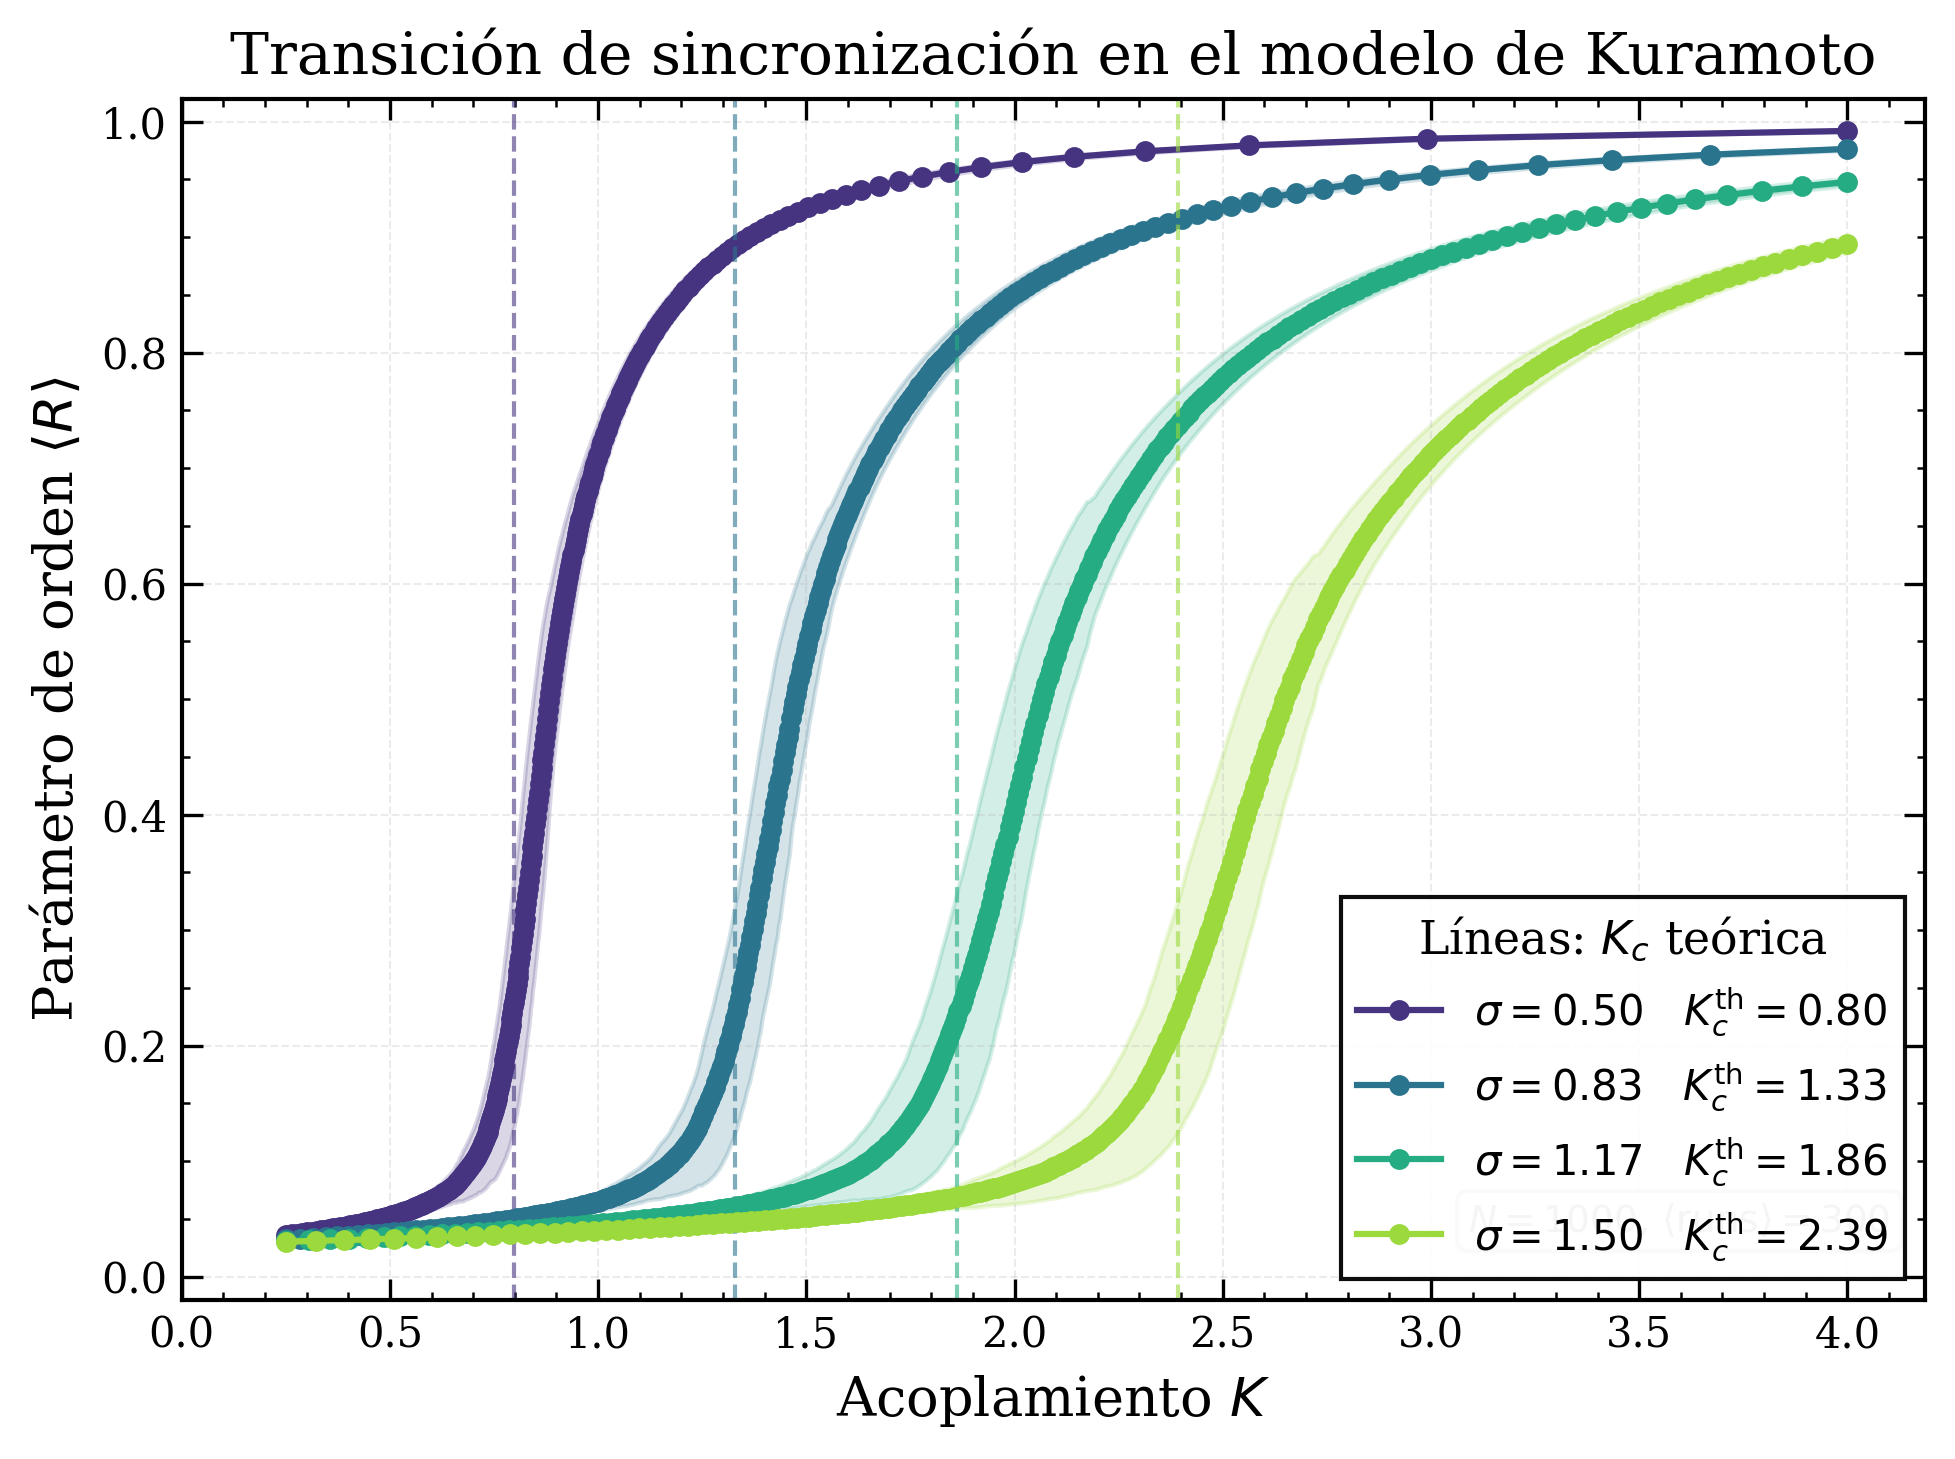
\includegraphics[width=0.45\textwidth]{R_vs_K.png}\hfill
  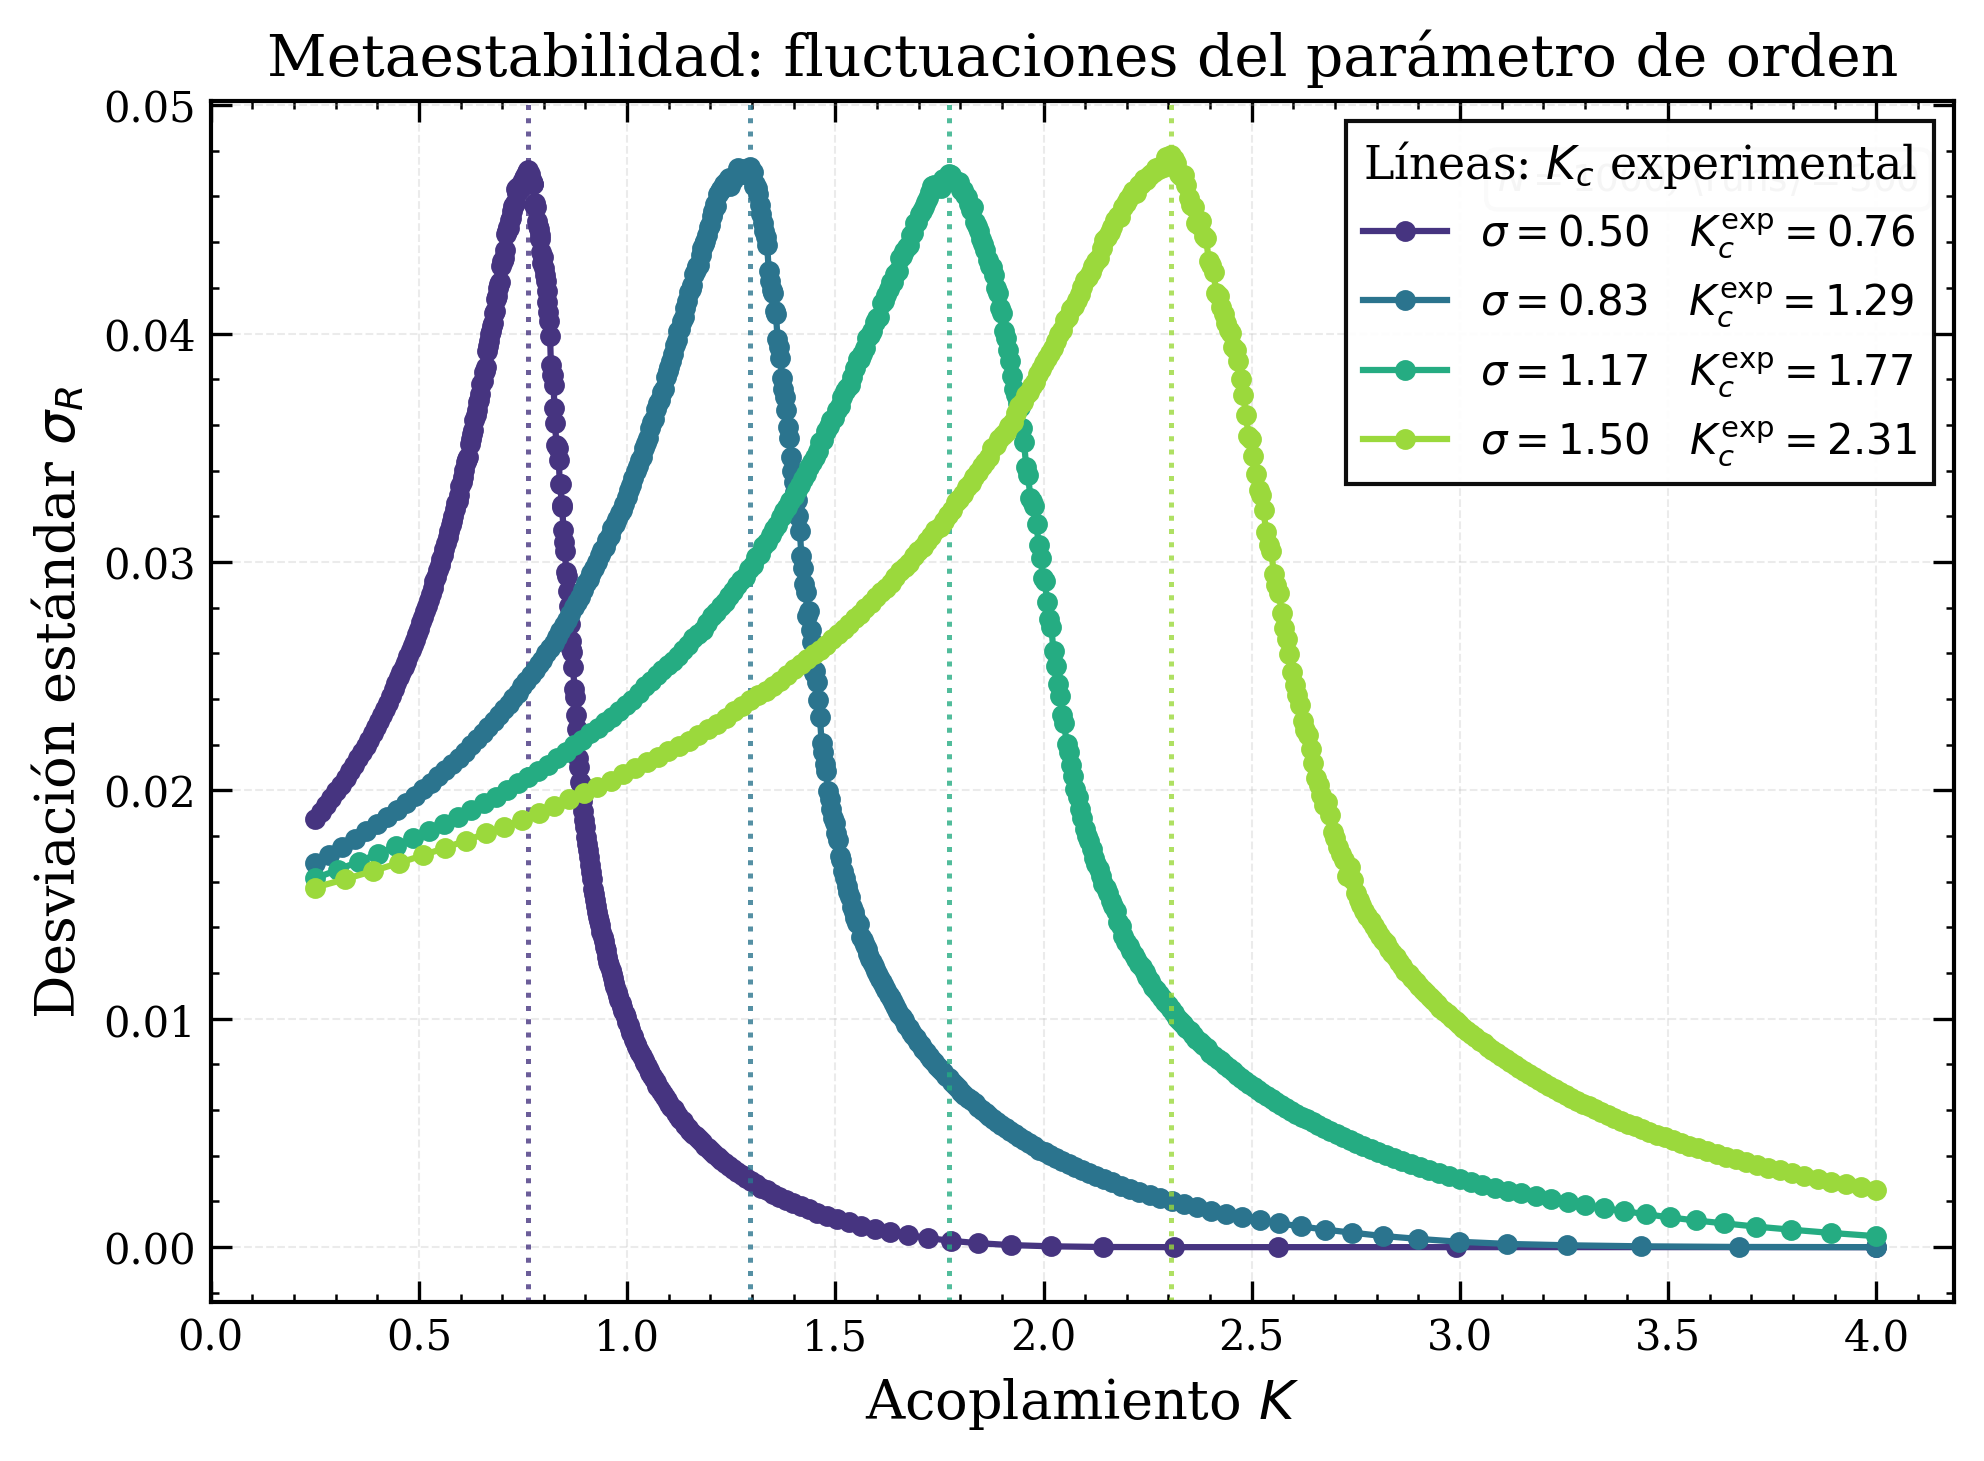
\includegraphics[width=0.45\textwidth]{sigmaR_vs_K.png}
  \caption{Transición clásica de Kuramoto en campo medio ($N=1000$ osciladores, 300 realizaciones, $t_{\max}=1000$, $dt=0.025$). Izquierda: promedio del parámetro de orden global $\langle R\rangle$ frente a $K$, junto a los valores de $K_c$ teóricos, para distintos valores de $\sigma$. Derecha: desviación estándar de $R$, $\sigma_R$, frente a $K$, junto a los $K_c$ experimentales obtenidos como el máximo de $\sigma_R$ (mayor fluctuación del parámetro de orden), para los mismos valores de $\sigma$.}
  \label{fig:tarea1}
\end{figure*}

En la \cref{fig:tarea3_scaling} se muestra el análisis de escalado de tamaño finito, extrapolando $K_c(N)$ al límite termodinámico $N\to \infty$ mediante una ley de potencias del tipo $K_c(N)=K_c^\infty+aN^{-\alpha}$ para $\alpha=1$ (izquierda) y $\alpha=2/5$ (derecha). Se puede ver que los resultados más satisfactorios se obtienen con $\alpha=2/5$, obteniendo errores relativos por debajo del $0.7\%$ (mientras que los errores relativos en el primer caso rondan el $3-4\%$), confirmando la tendencia propuesta por Hong \textit{et al.}~\cite{hong2007finite}.

\begin{figure*}[t]
  \centering
  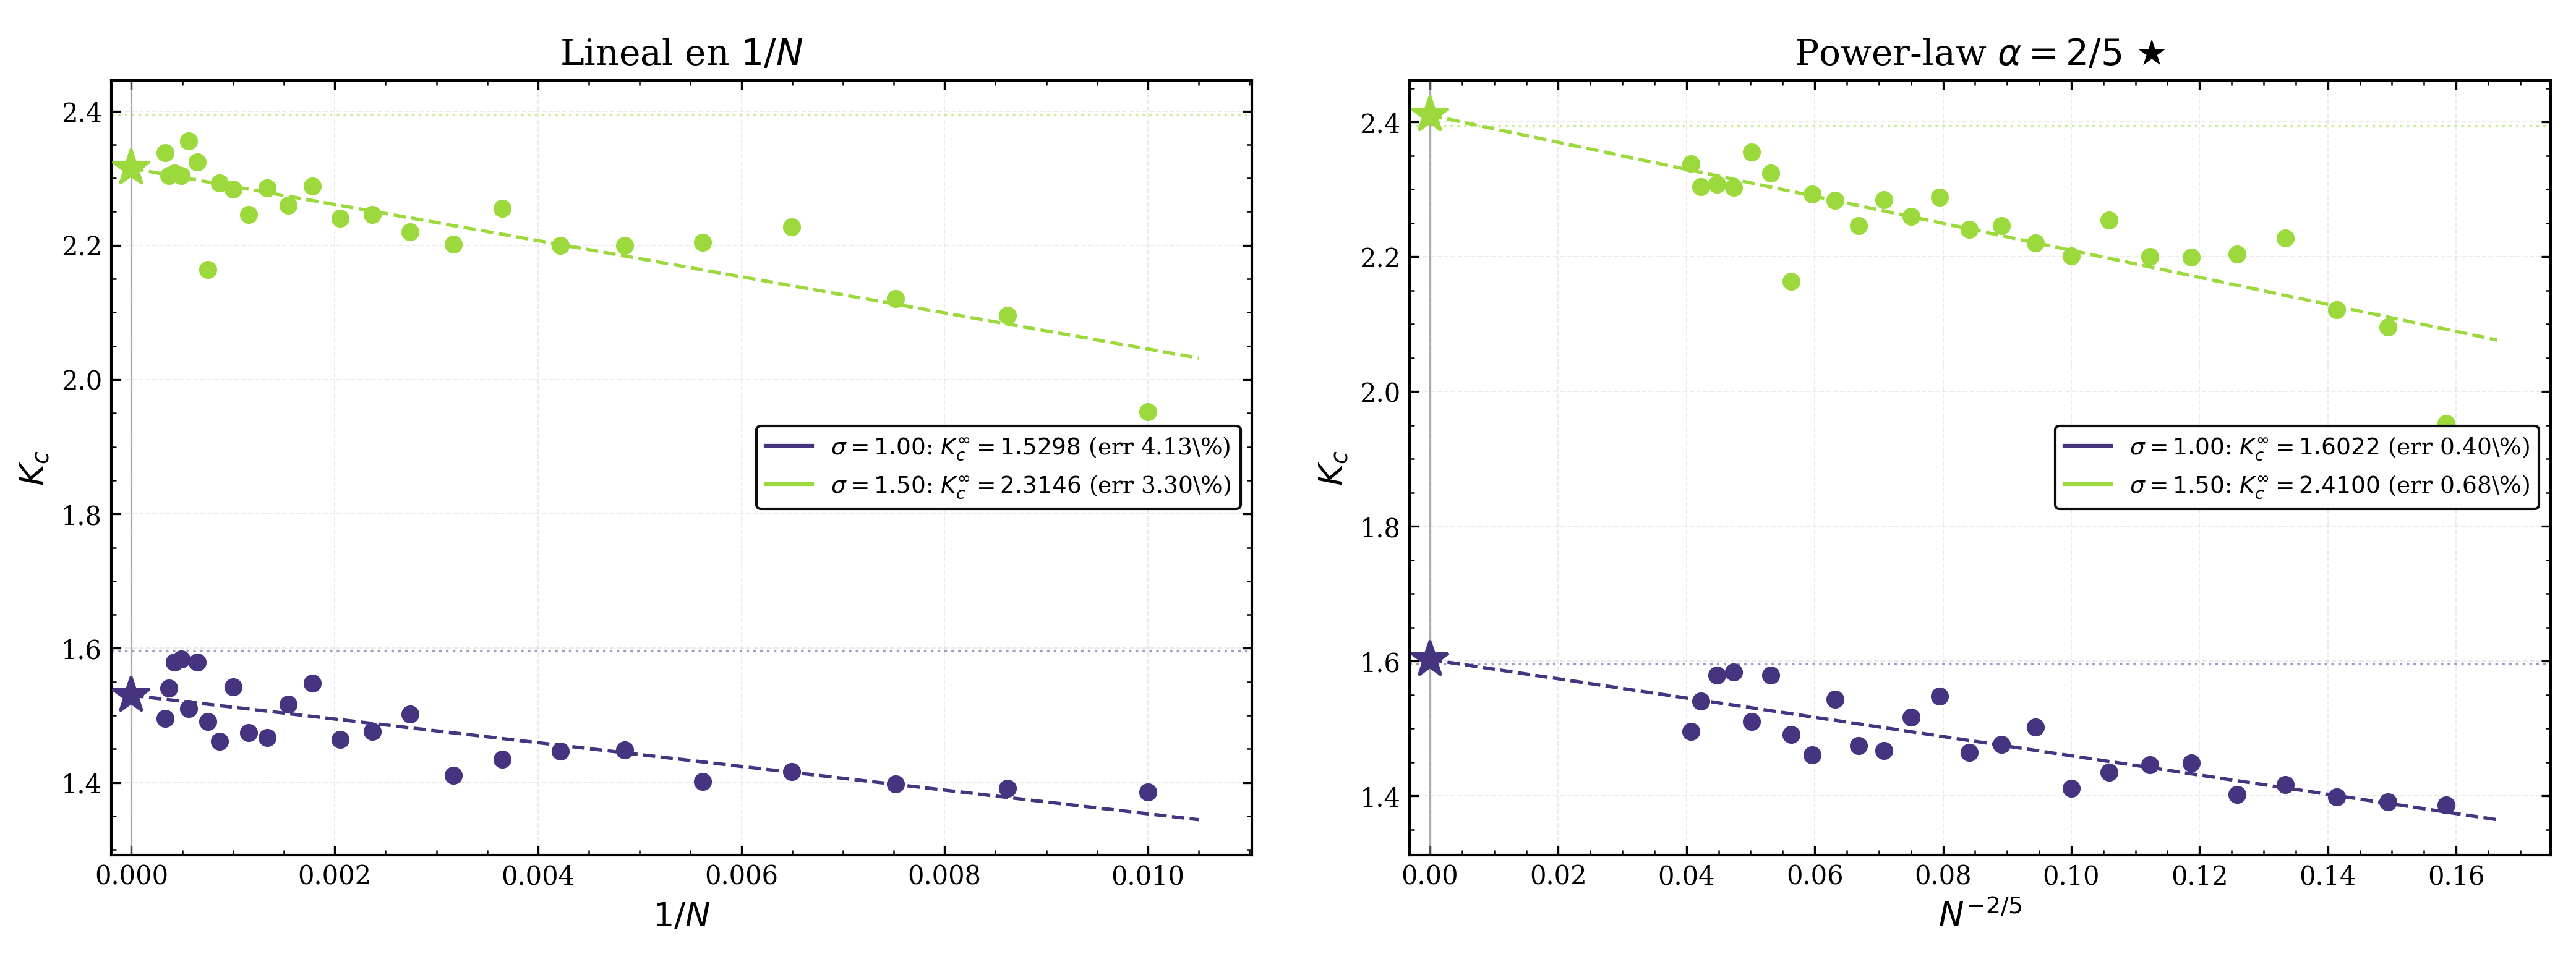
\includegraphics[width=0.9\textwidth]{scaling_Kc2.png}
  \caption{Extrapolación de $K_c(N)$ al límite termodinámico mediante la ley de potencias $K_c(N)=K_c^\infty+aN^{-\alpha}$. Izquierda: $\alpha=1$. Derecha: $\alpha=2/5$. Resultados obtenidos para $\sigma=1$ (azul) y $\sigma=1.5$ (verde). En la leyenda se muestran los valores de $K_c^\infty$ obtenidos y su error relativo.}
  \label{fig:tarea3_scaling}
\end{figure*}


\subsection{Tarea 2: Red modular}
\label{sec:tarea2}

El modelo de campo medio está muy alejado de cómo son las redes neuronales reales y no es capaz de predecir muchos de los fenómenos físicos que se observan. Una mejor aproximación~\cite{villegas2014frustrated} consiste en suponer una red compuesta por dos módulos densamente conectados internamente (todos conectados entre sí), pero débilmente conectados entre sí (una única conexión entre ellos). Con este modelo, el sistema es capaz de explicar el régimen de metaestabilidad, donde cada módulo se sincroniza internamente ($r_m\approx 1$), pero la débil conexión inter-modular es incapaz de imponer un orden global. Como consecuencia de esta frustración, el sistema entra en un régimen donde el parámetro de orden global no alcanza un estado estacionario, sino que exhibe grandes fluctuaciones sostenidas.

Para entender mejor este fenómeno, resulta útil plantear la siguiente analogía: imaginemos dos habitaciones separadas (los módulos), ambas llenas de personas (osciladores) que aplauden, cada una a su propio ritmo natural (frecuencia intrínseca). El acoplamiento global $K$ representa la predisposición general de las personas a ajustar su aplauso al de los demás. Al aumentar $K$, la alta densidad de personas dentro de una misma sala hace que sus aplausos se sincronicen rápidamente. La conexión débil inter-modular equivaldría a tener a una sola persona de cada habitación conectada con la otra mediante una llamada telefónica. El régimen de metaestabilidad es precisamente aquel rango de $K$ donde el acoplamiento es lo suficientemente fuerte para que cada habitación mantenga su sincronización interna, pero la influencia transmitida a través de esa única llamada es insuficiente para vencer la diferencia de ritmos entre ambas salas. Como resultado, las habitaciones intentan acoplarse, se adelantan o se atrasan, y nunca logran sincronizarse entre sí de manera continua, generando así las fluctuaciones macroscópicas observadas.

En la \cref{fig:tarea2} se puede observar el régimen de metaestabilidad mencionado, donde los módulos están sincronizados internamente ($r_1\approx r_2 \approx 1$) pero no hay coherencia total global ($R\neq 1$). Para valores de $K$ muy pequeños, la red no es capaz ni de sincronizarse internamente, y para valores de $K$ muy elevados, se sincroniza local y globalmente. El fenómeno de la metaestabilidad retrasa la coherencia total global.

Al comparar la curva de $\sigma_R$ con la obtenida para el caso de campo medio (\cref{fig:tarea1}), se observa cómo el pico estrecho original se ha ensanchado significativamente, dando lugar a una región extendida de metaestabilidad. Por su parte, las curvas de $\sigma_{r_1}$ y $\sigma_{r_2}$ son similares a la del modelo de campo medio (internamente están densamente conectados).

\begin{figure*}[t]
  \centering
  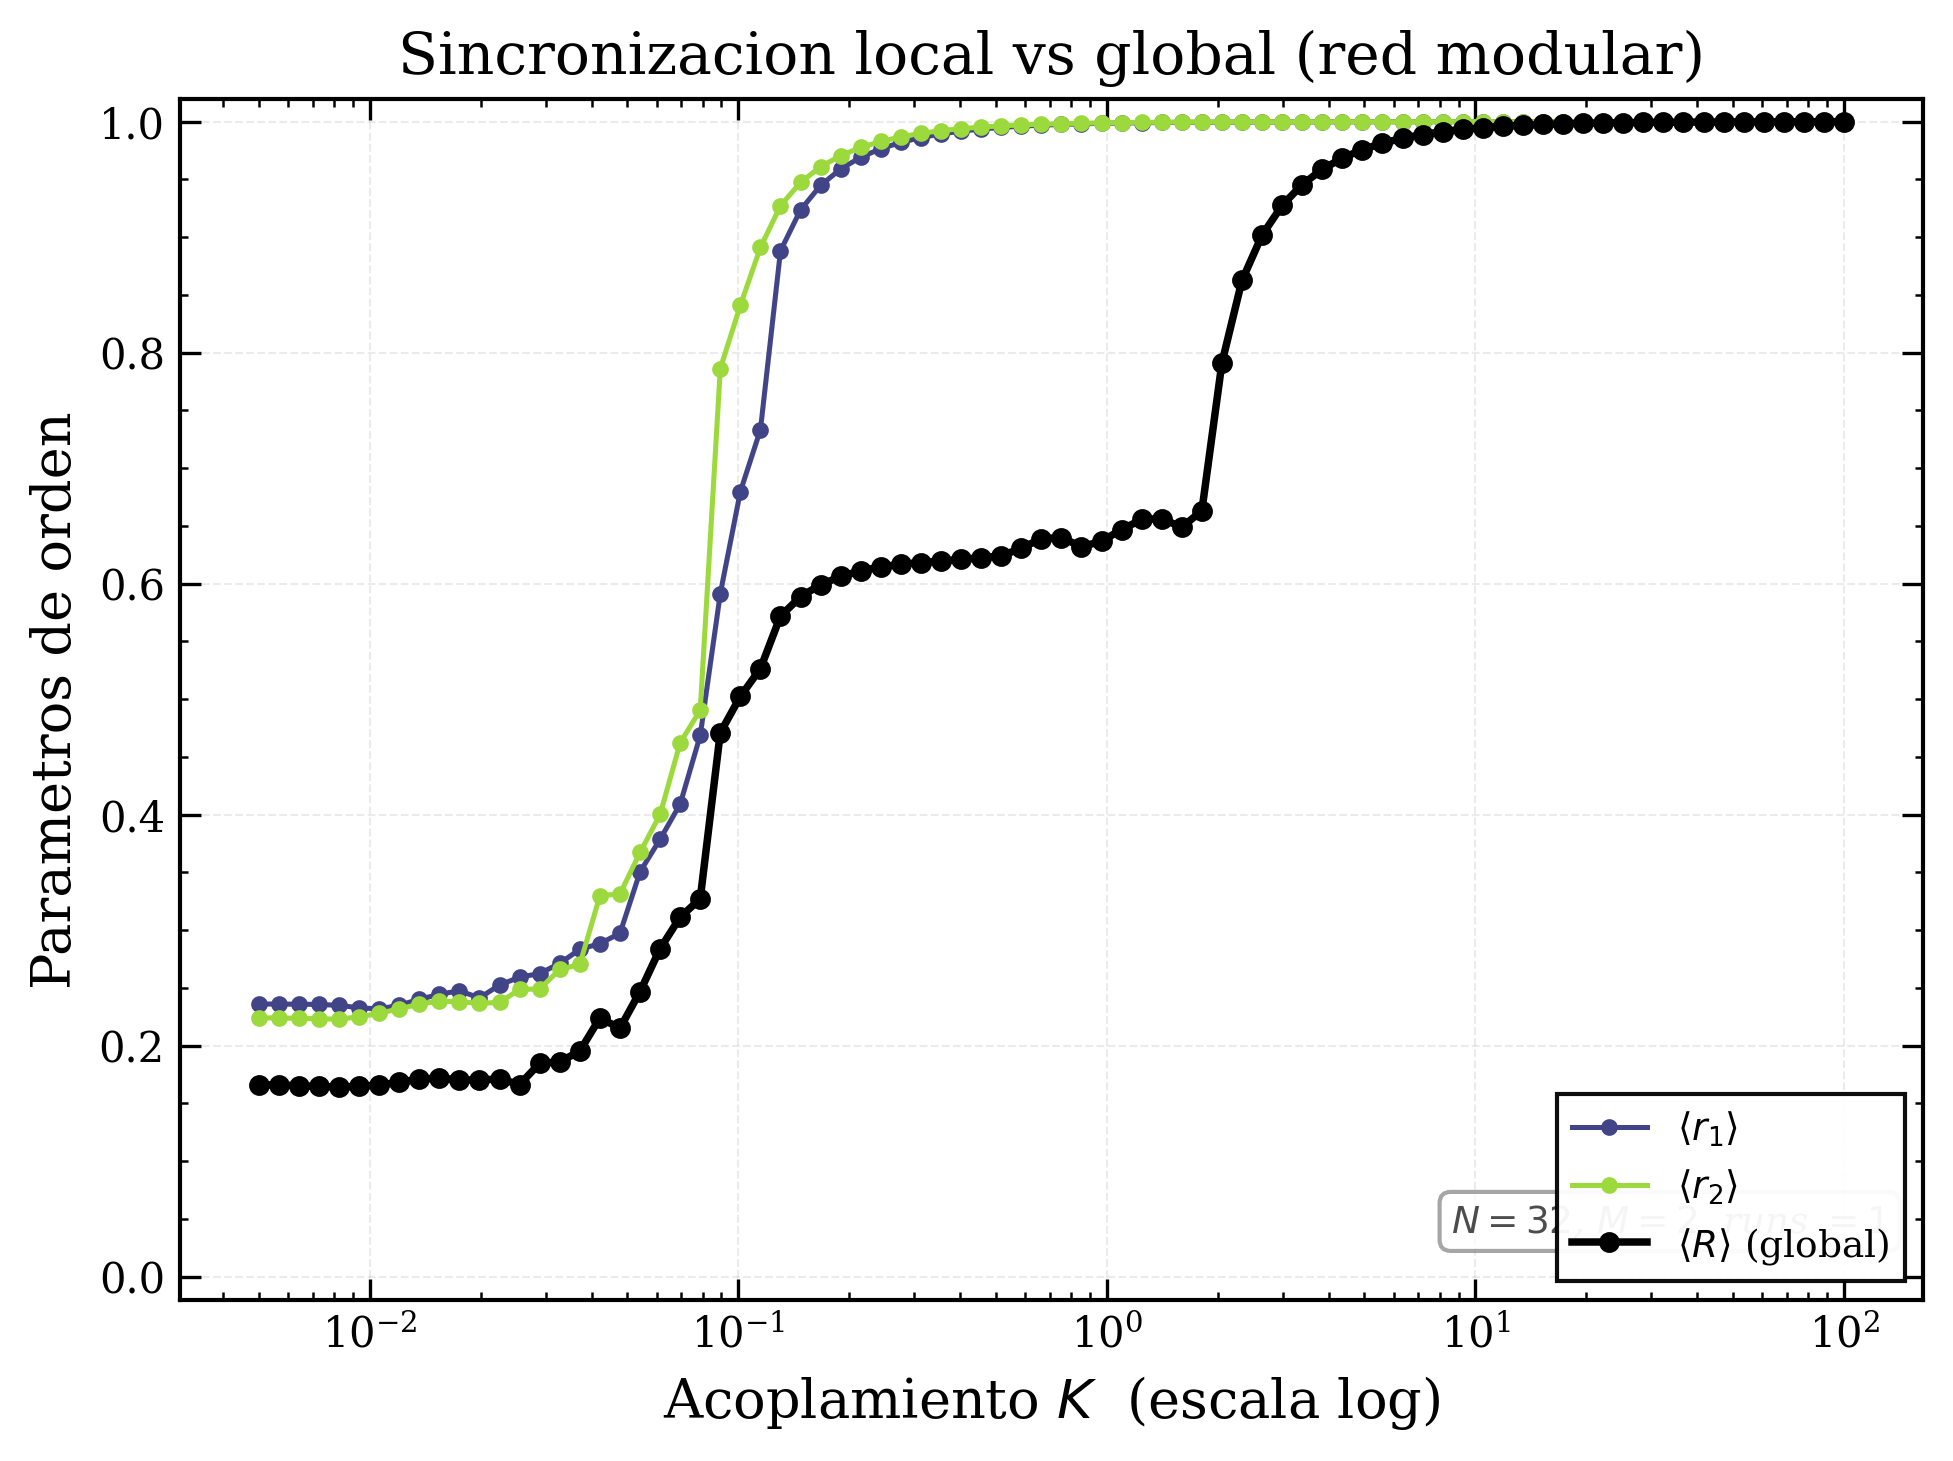
\includegraphics[width=0.45\textwidth]{SincMod.png}\hfill
  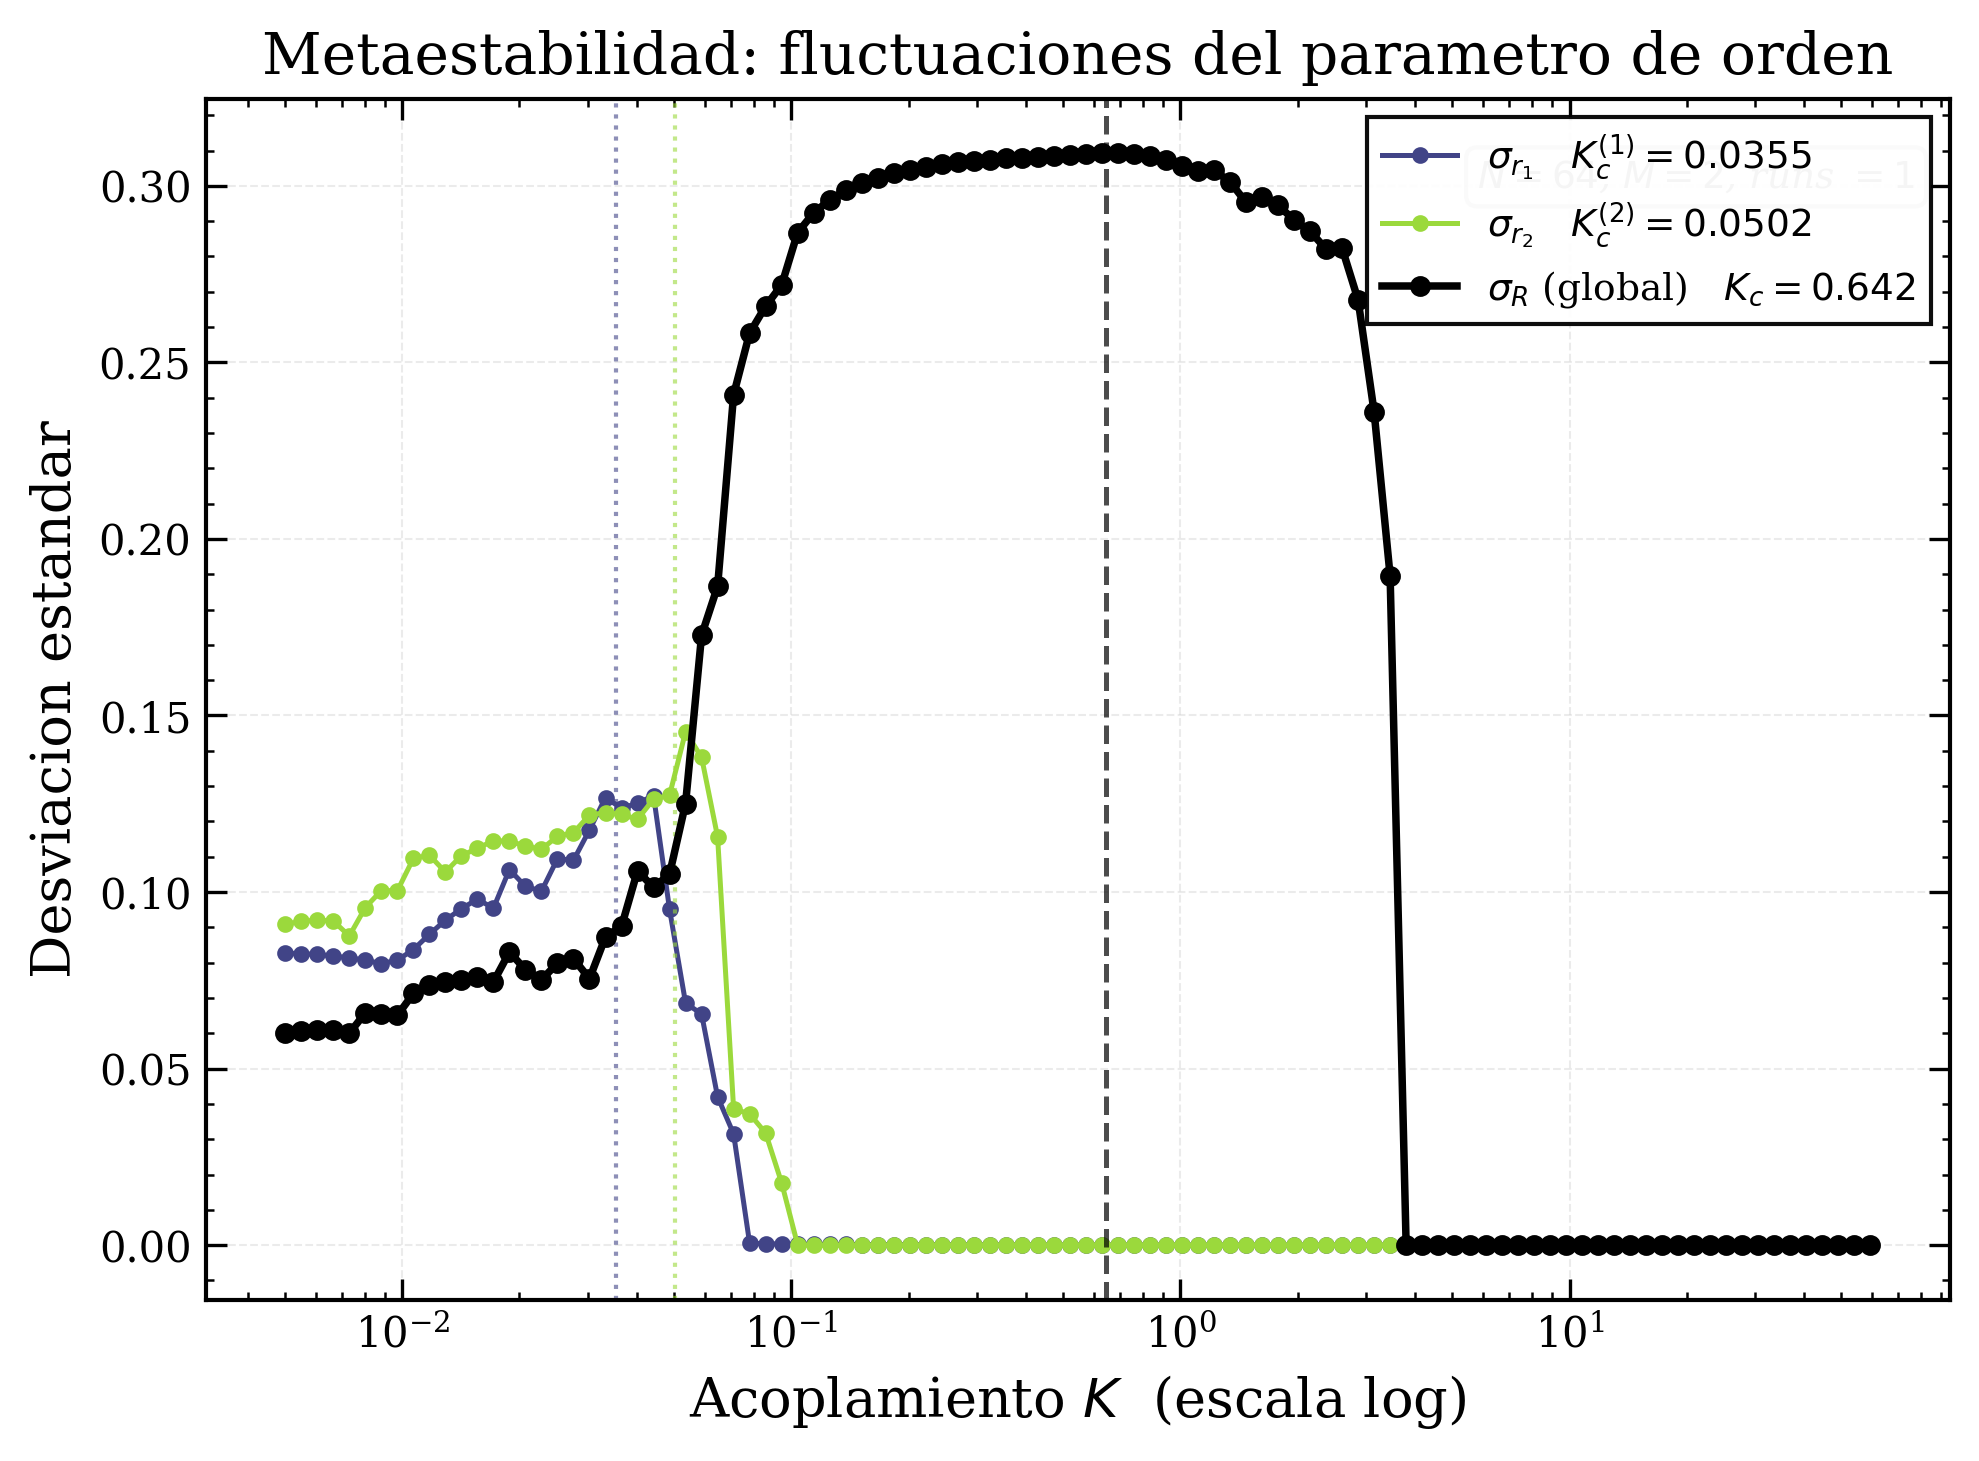
\includegraphics[width=0.45\textwidth]{sigmar1r2R.png}
  \caption{Red modular ($N=32$ osciladores, $m=2$ módulos). Izquierda: en negro, promedio del parámetro de orden global $\langle R\rangle$ frente a $K$; en azul y verde, promedio de los parámetros de orden locales $\langle r_1\rangle$ y $\langle r_2\rangle$, respectivamente. Derecha: en negro, desviación estándar del parámetro de orden global $\sigma_R$ frente a $K$; en azul y verde, desviaciones estándar de los parámetros de orden locales $\sigma_{r_1}$ y $\sigma_{r_2}$, respectivamente.}
  \label{fig:tarea2}
\end{figure*}

\subsection{Tarea 3: Estructura jerárquica}
\label{sec:tarea3}

Se pueden reproducir de una forma más fiable los resultados de las redes neuronales reales si consideramos que el número de módulos es mayor y que puede haber una estructura jerárquica, con módulos dentro de módulos. En este tipo de redes, la coherencia emerge de forma escalonada: la sincronización se consolida primero en los niveles más locales y se propaga progresivamente hacia las escalas globales. Esto sucede principalmente porque las conexiones entre módulos de niveles más bajos son más frecuentes que las de los módulos más externos.

En las Figuras \ref{fig:tarea3_modulos_12} y \ref{fig:tarea3_modulo3_A} se muestran las gráficas de parámetro de orden locales (nivel 2) y globales (nivel 1) para los 3 módulos principales. Se observan curvas similares a las obtenidas en la red modular no jerárquica (véase \cref{fig:tarea2}).

En la \cref{fig:tarea3_global} se puede ver claramente cómo el aumento del orden global se produce de manera escalonada, emergiendo primero la coherencia en los niveles más locales y sincronizándose poco a poco en niveles más globales, dando lugar a varias mesetas de estabilidad (metaestabilidad). La desviación estándar del parámetro de orden global ya no presenta ni un pico estrecho ni una región plana extendida, sino una sucesión de subidas y bajas alrededor de una misma altura. Se aprecia, de nuevo, que los máximos de las distribuciones locales se dan antes (menores valores de $K$) que el global.

\begin{figure*}[t]
  \centering
  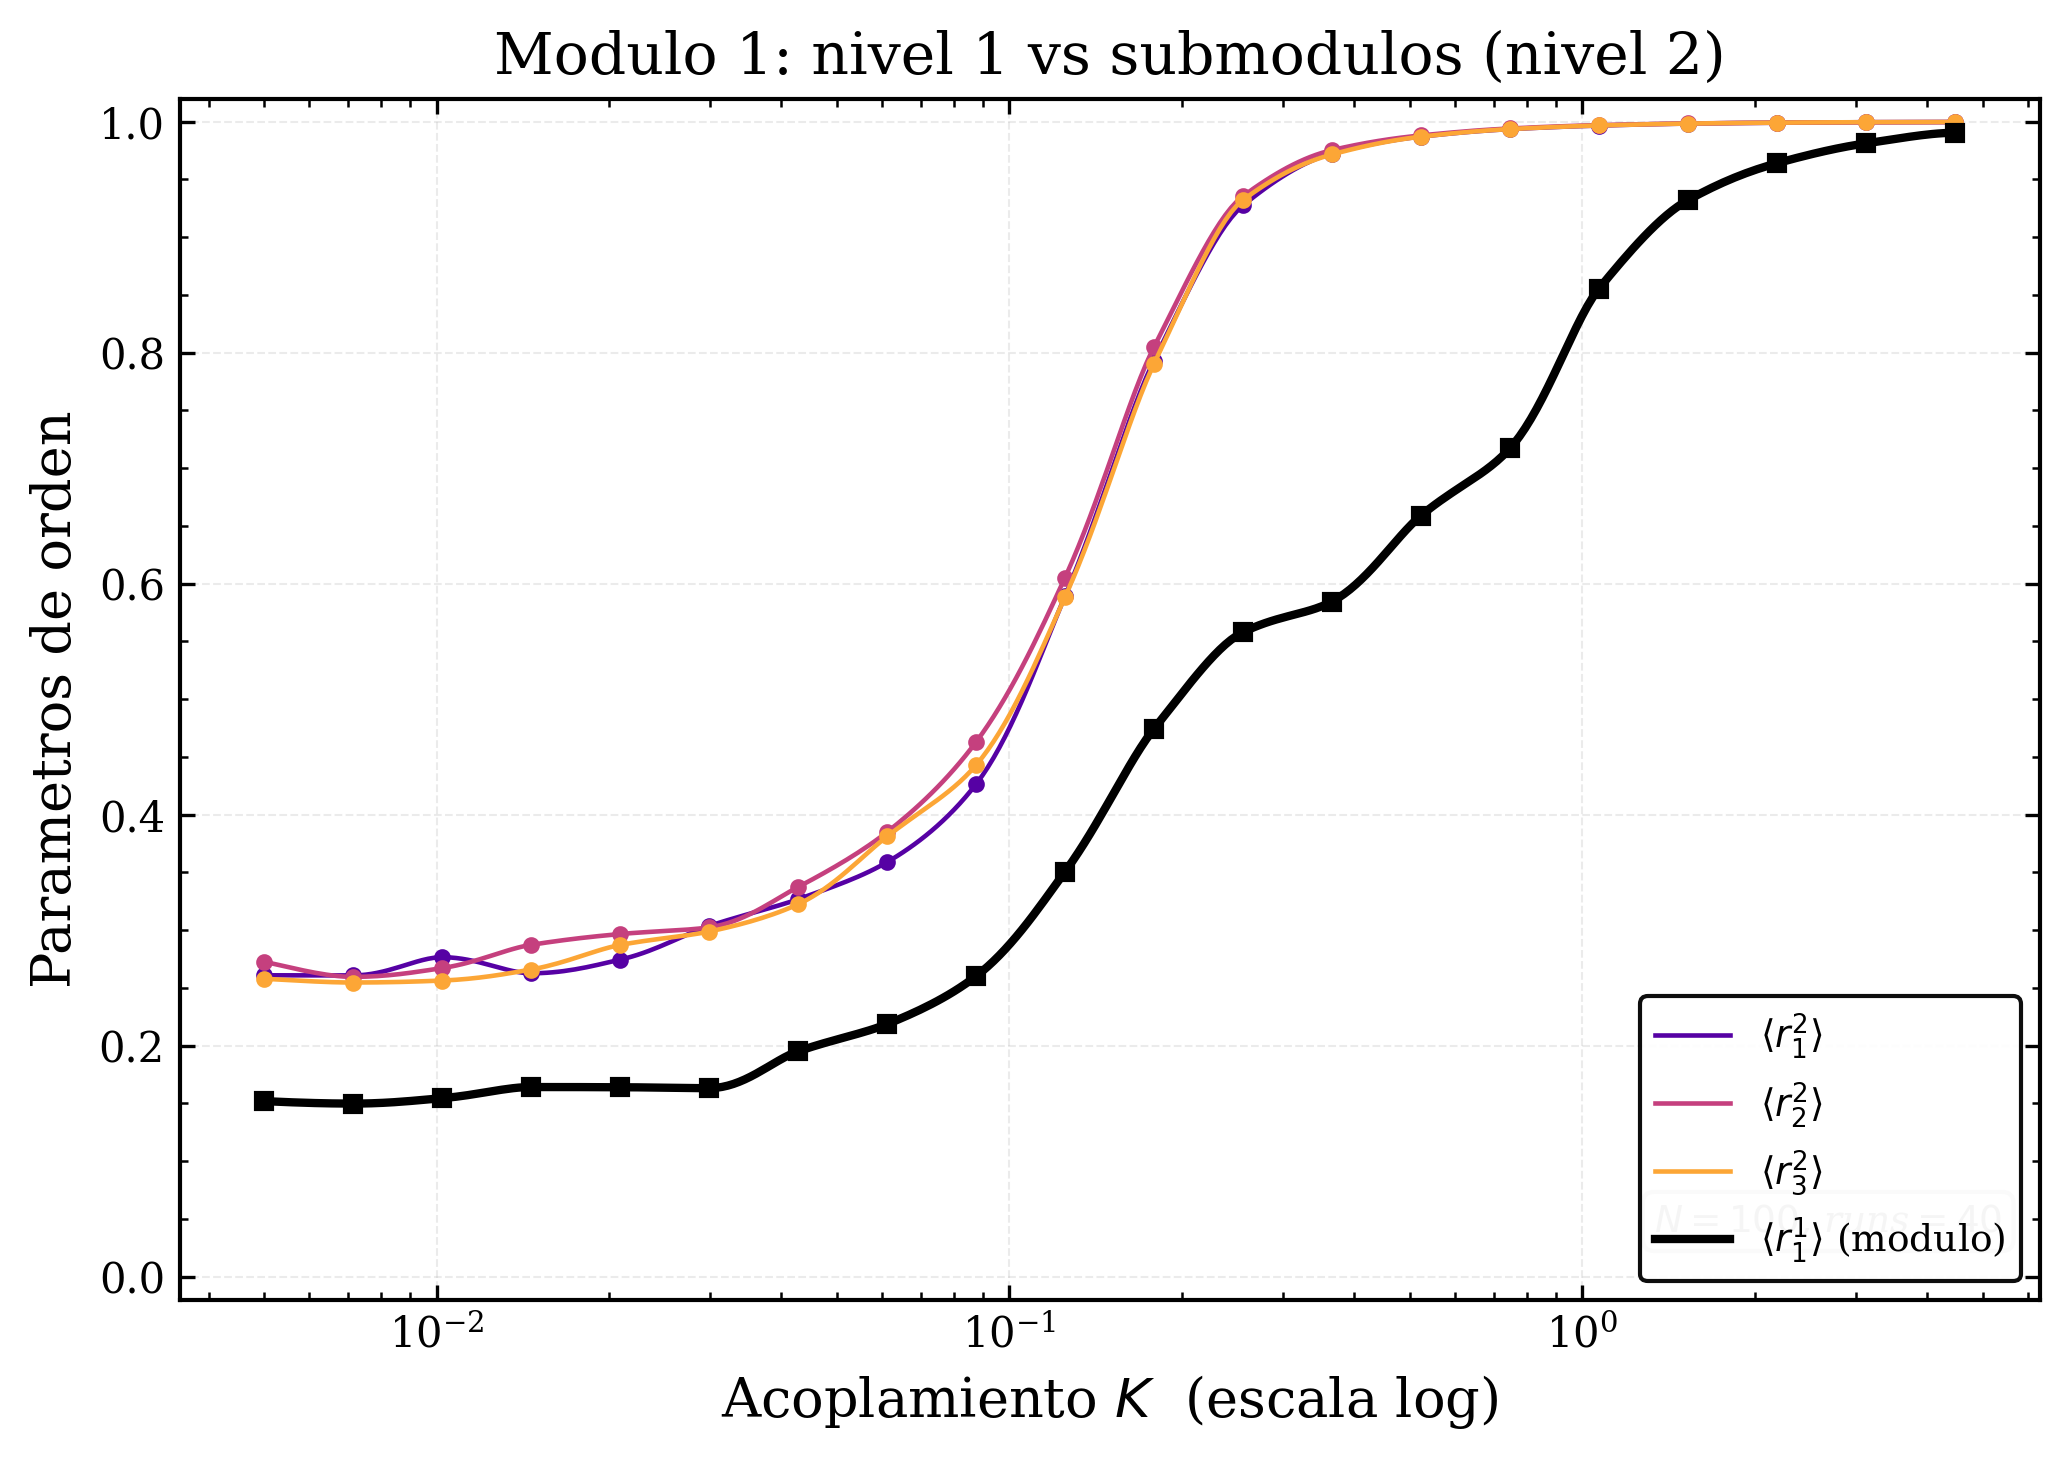
\includegraphics[width=0.45\textwidth]{modulo_1.png}\hfill
  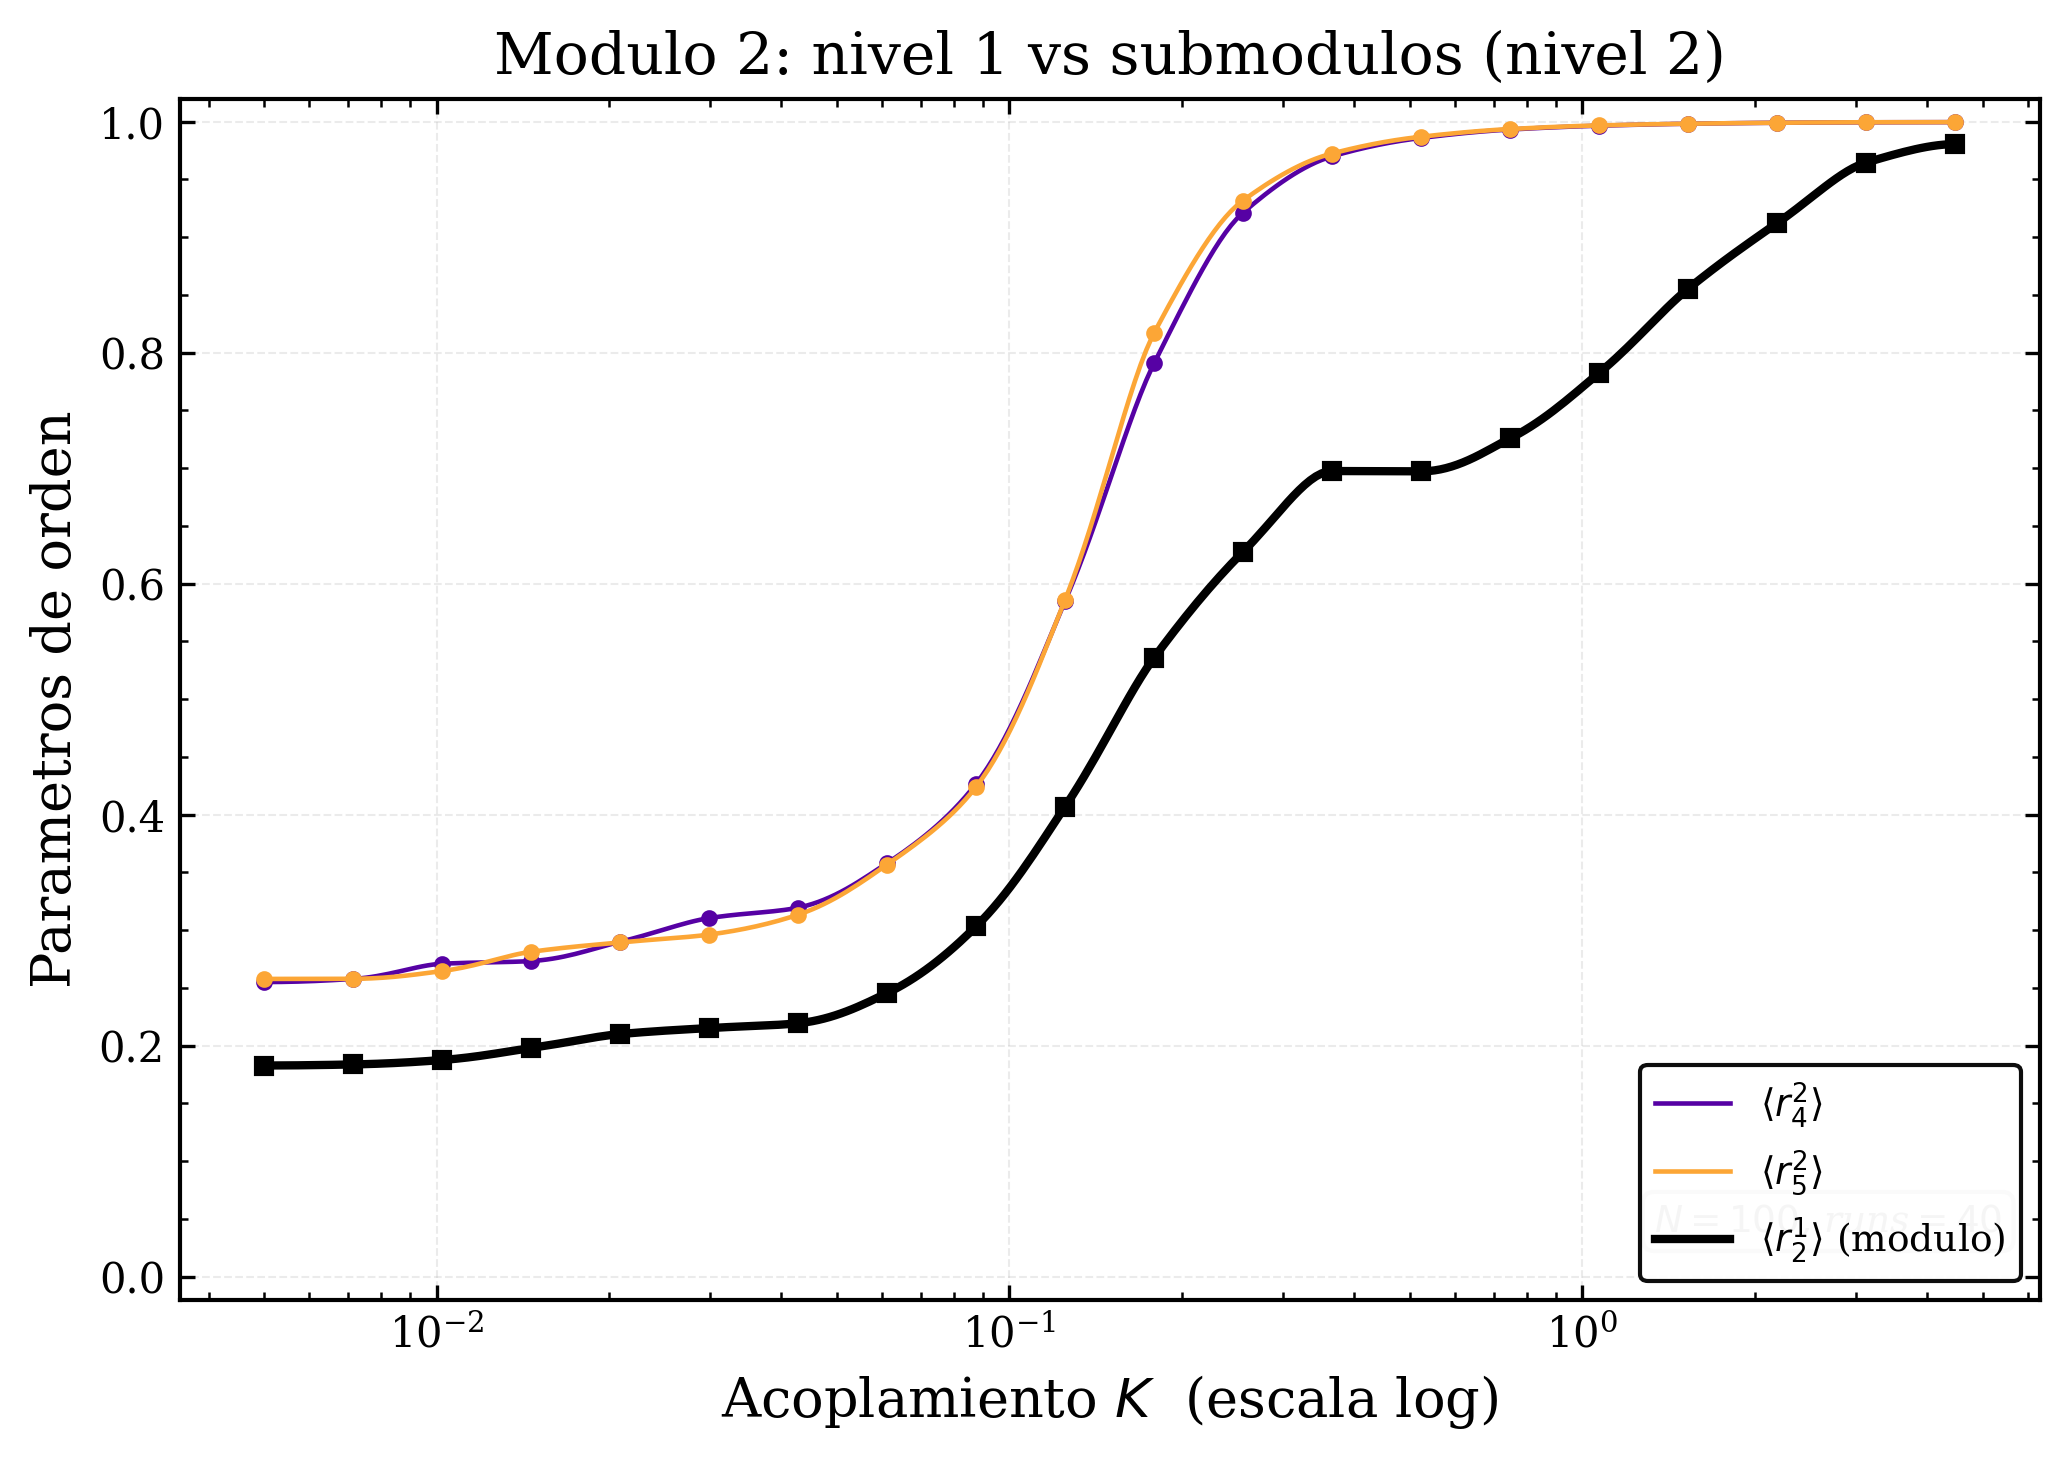
\includegraphics[width=0.45\textwidth]{modulo_2.png}
  \caption{Red jerárquica ($N=100$ osciladores, $m=3$ módulos de nivel 1, 8 submódulos de nivel 2). Izquierda: primer módulo --- en negro, promedio del parámetro de orden del módulo (nivel 1), $\langle r_1^1\rangle$, frente a $K$; en morado, rosa y naranja, parámetros de orden de los submódulos (nivel 2) $\langle r^2_1\rangle$, $\langle r^2_2\rangle$ y $\langle r^2_3\rangle$. Derecha: segundo módulo --- en negro, $\langle r_2^1\rangle$ frente a $K$; en morado y naranja, $\langle r^2_4\rangle$ y $\langle r^2_5\rangle$.}
  \label{fig:tarea3_modulos_12}
\end{figure*}

\begin{figure*}[t]
  \centering
  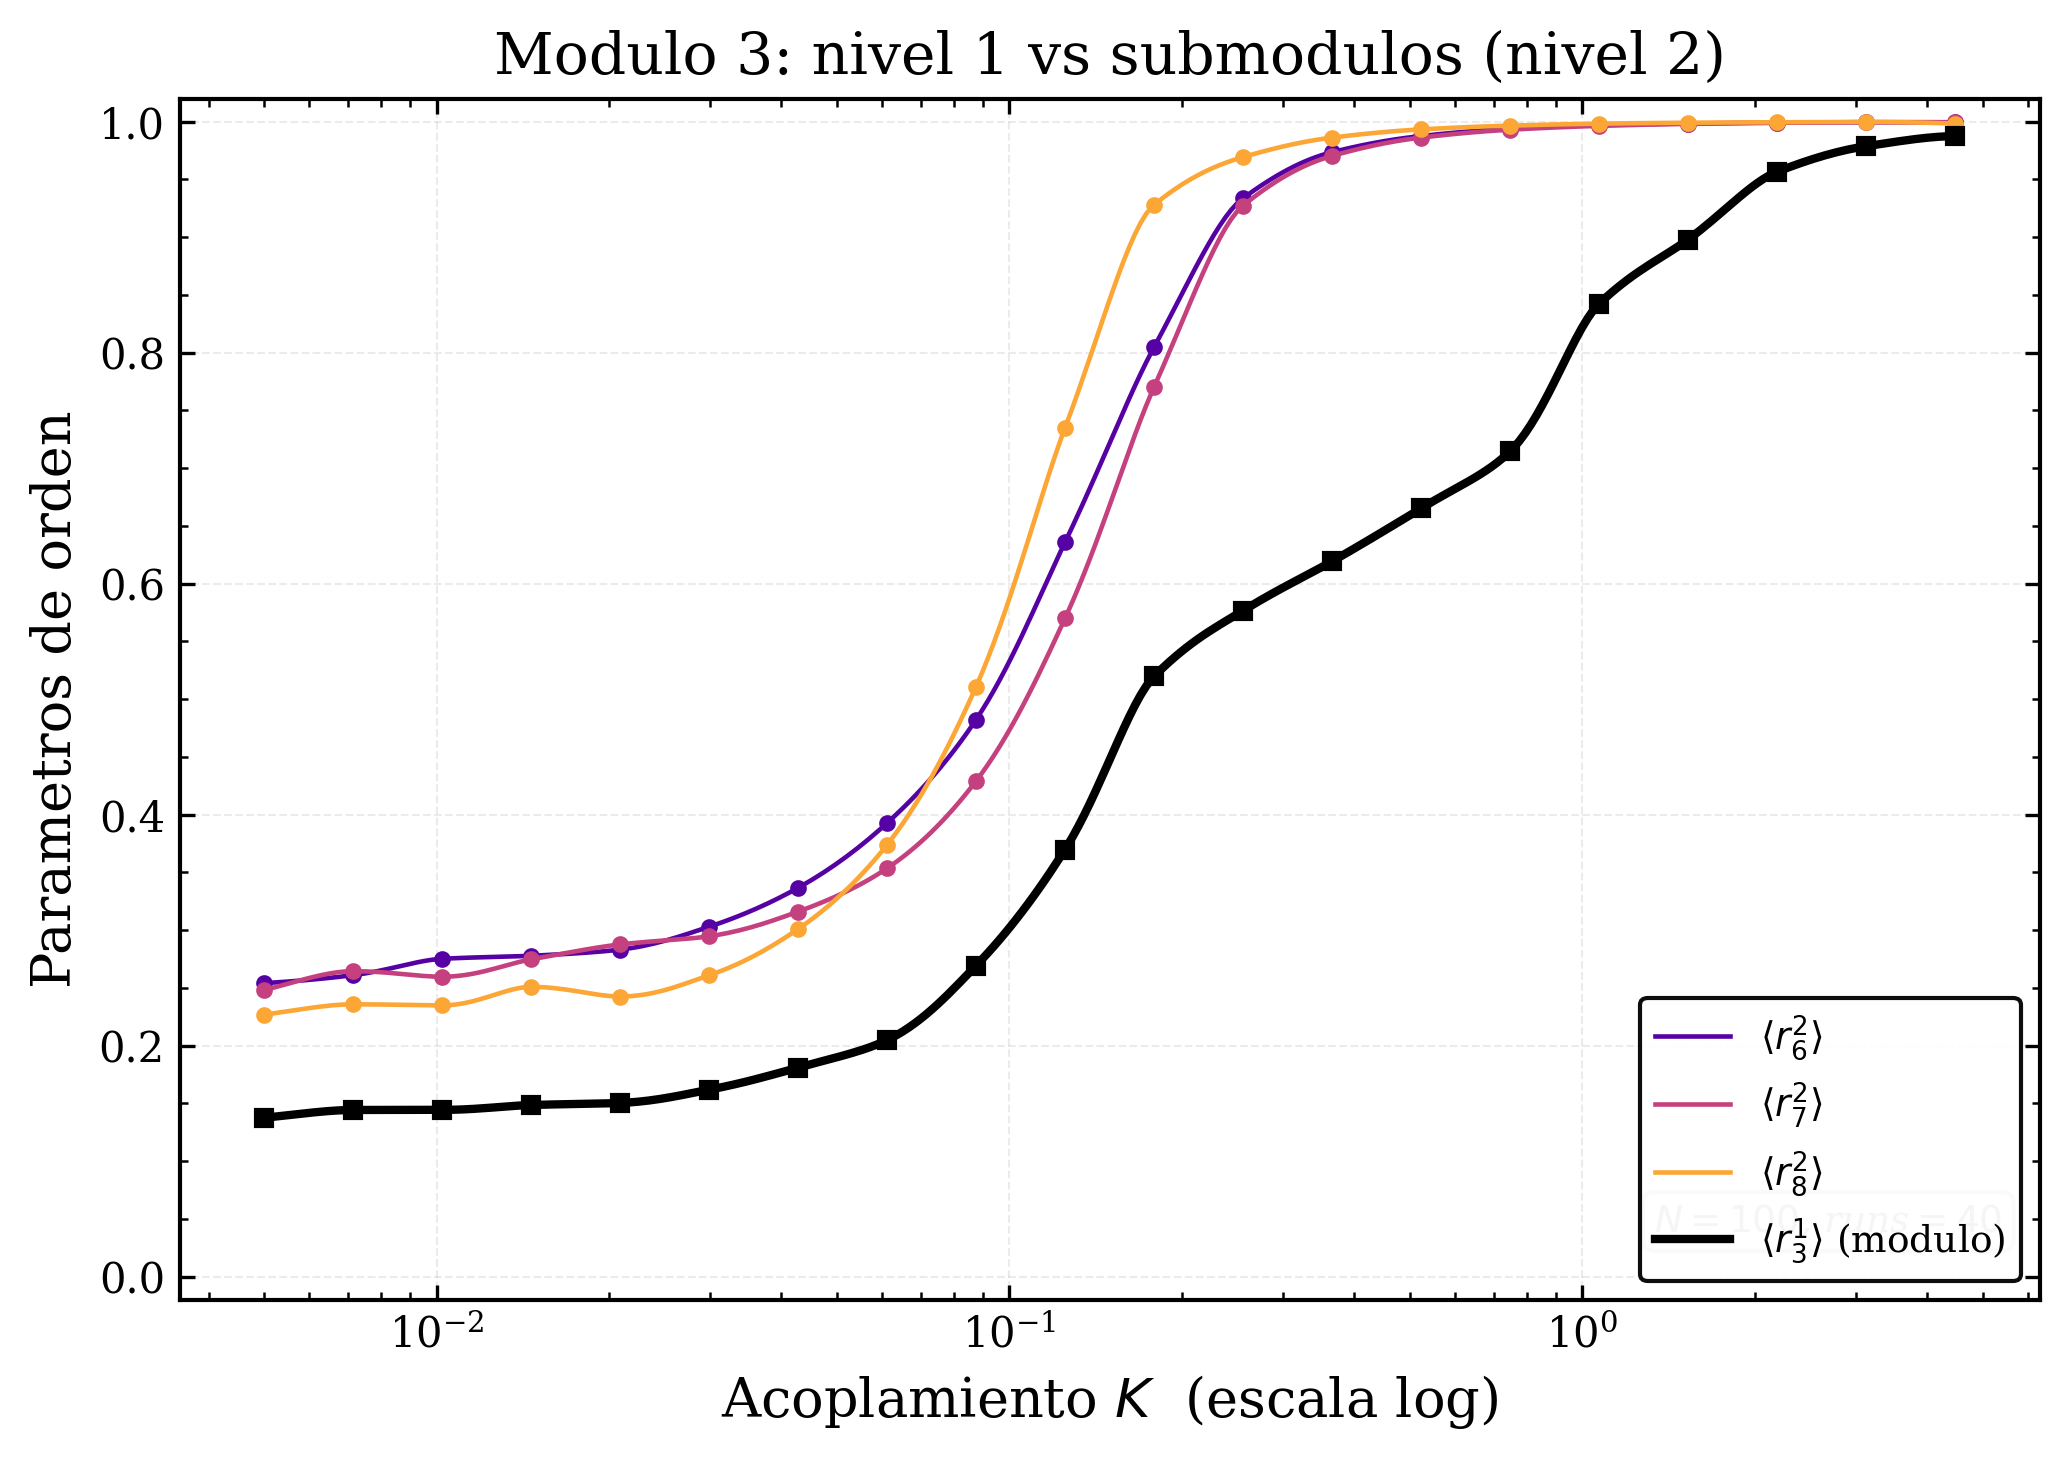
\includegraphics[width=0.45\textwidth]{modulo_3.png}\hfill
  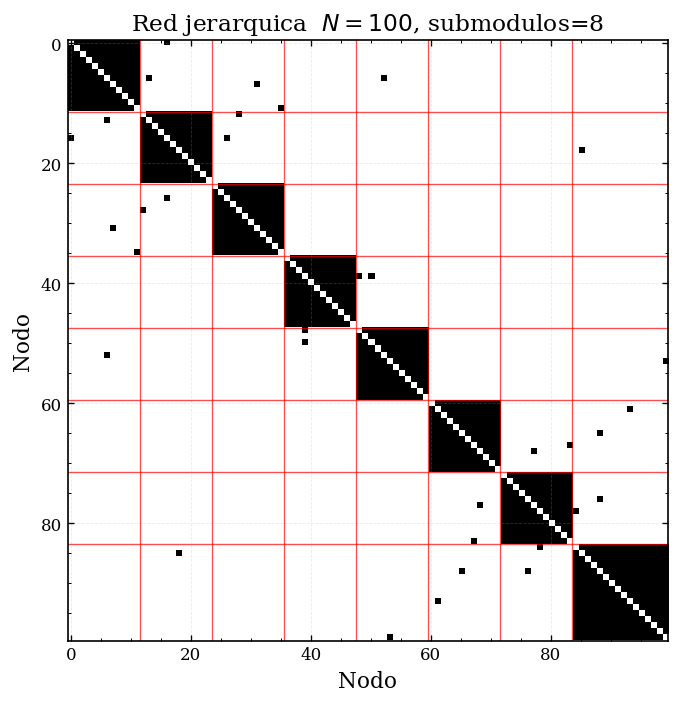
\includegraphics[width=0.45\textwidth]{A.png}
  \caption{Izquierda: tercer módulo --- en negro, promedio del parámetro de orden del módulo (nivel 1), $\langle r_3^1\rangle$, frente a $K$; en morado, rosa y naranja, parámetros de orden de los submódulos (nivel 2) $\langle r^2_6\rangle$, $\langle r^2_7\rangle$ y $\langle r^2_8\rangle$. Derecha: matriz de adyacencia utilizada para la Tarea~3. La estructura de la red consta de $m=3$ módulos (nivel 1), con $m_1=3$, $m_2=2$ y $m_3=3$ submódulos (nivel 2) respectivamente. Los módulos de nivel 1 están conectados entre sí por una única arista; los submódulos de un mismo módulo cuentan con 2 conexiones entre sí.}
  \label{fig:tarea3_modulo3_A}
\end{figure*}

\begin{figure*}[t]
  \centering
  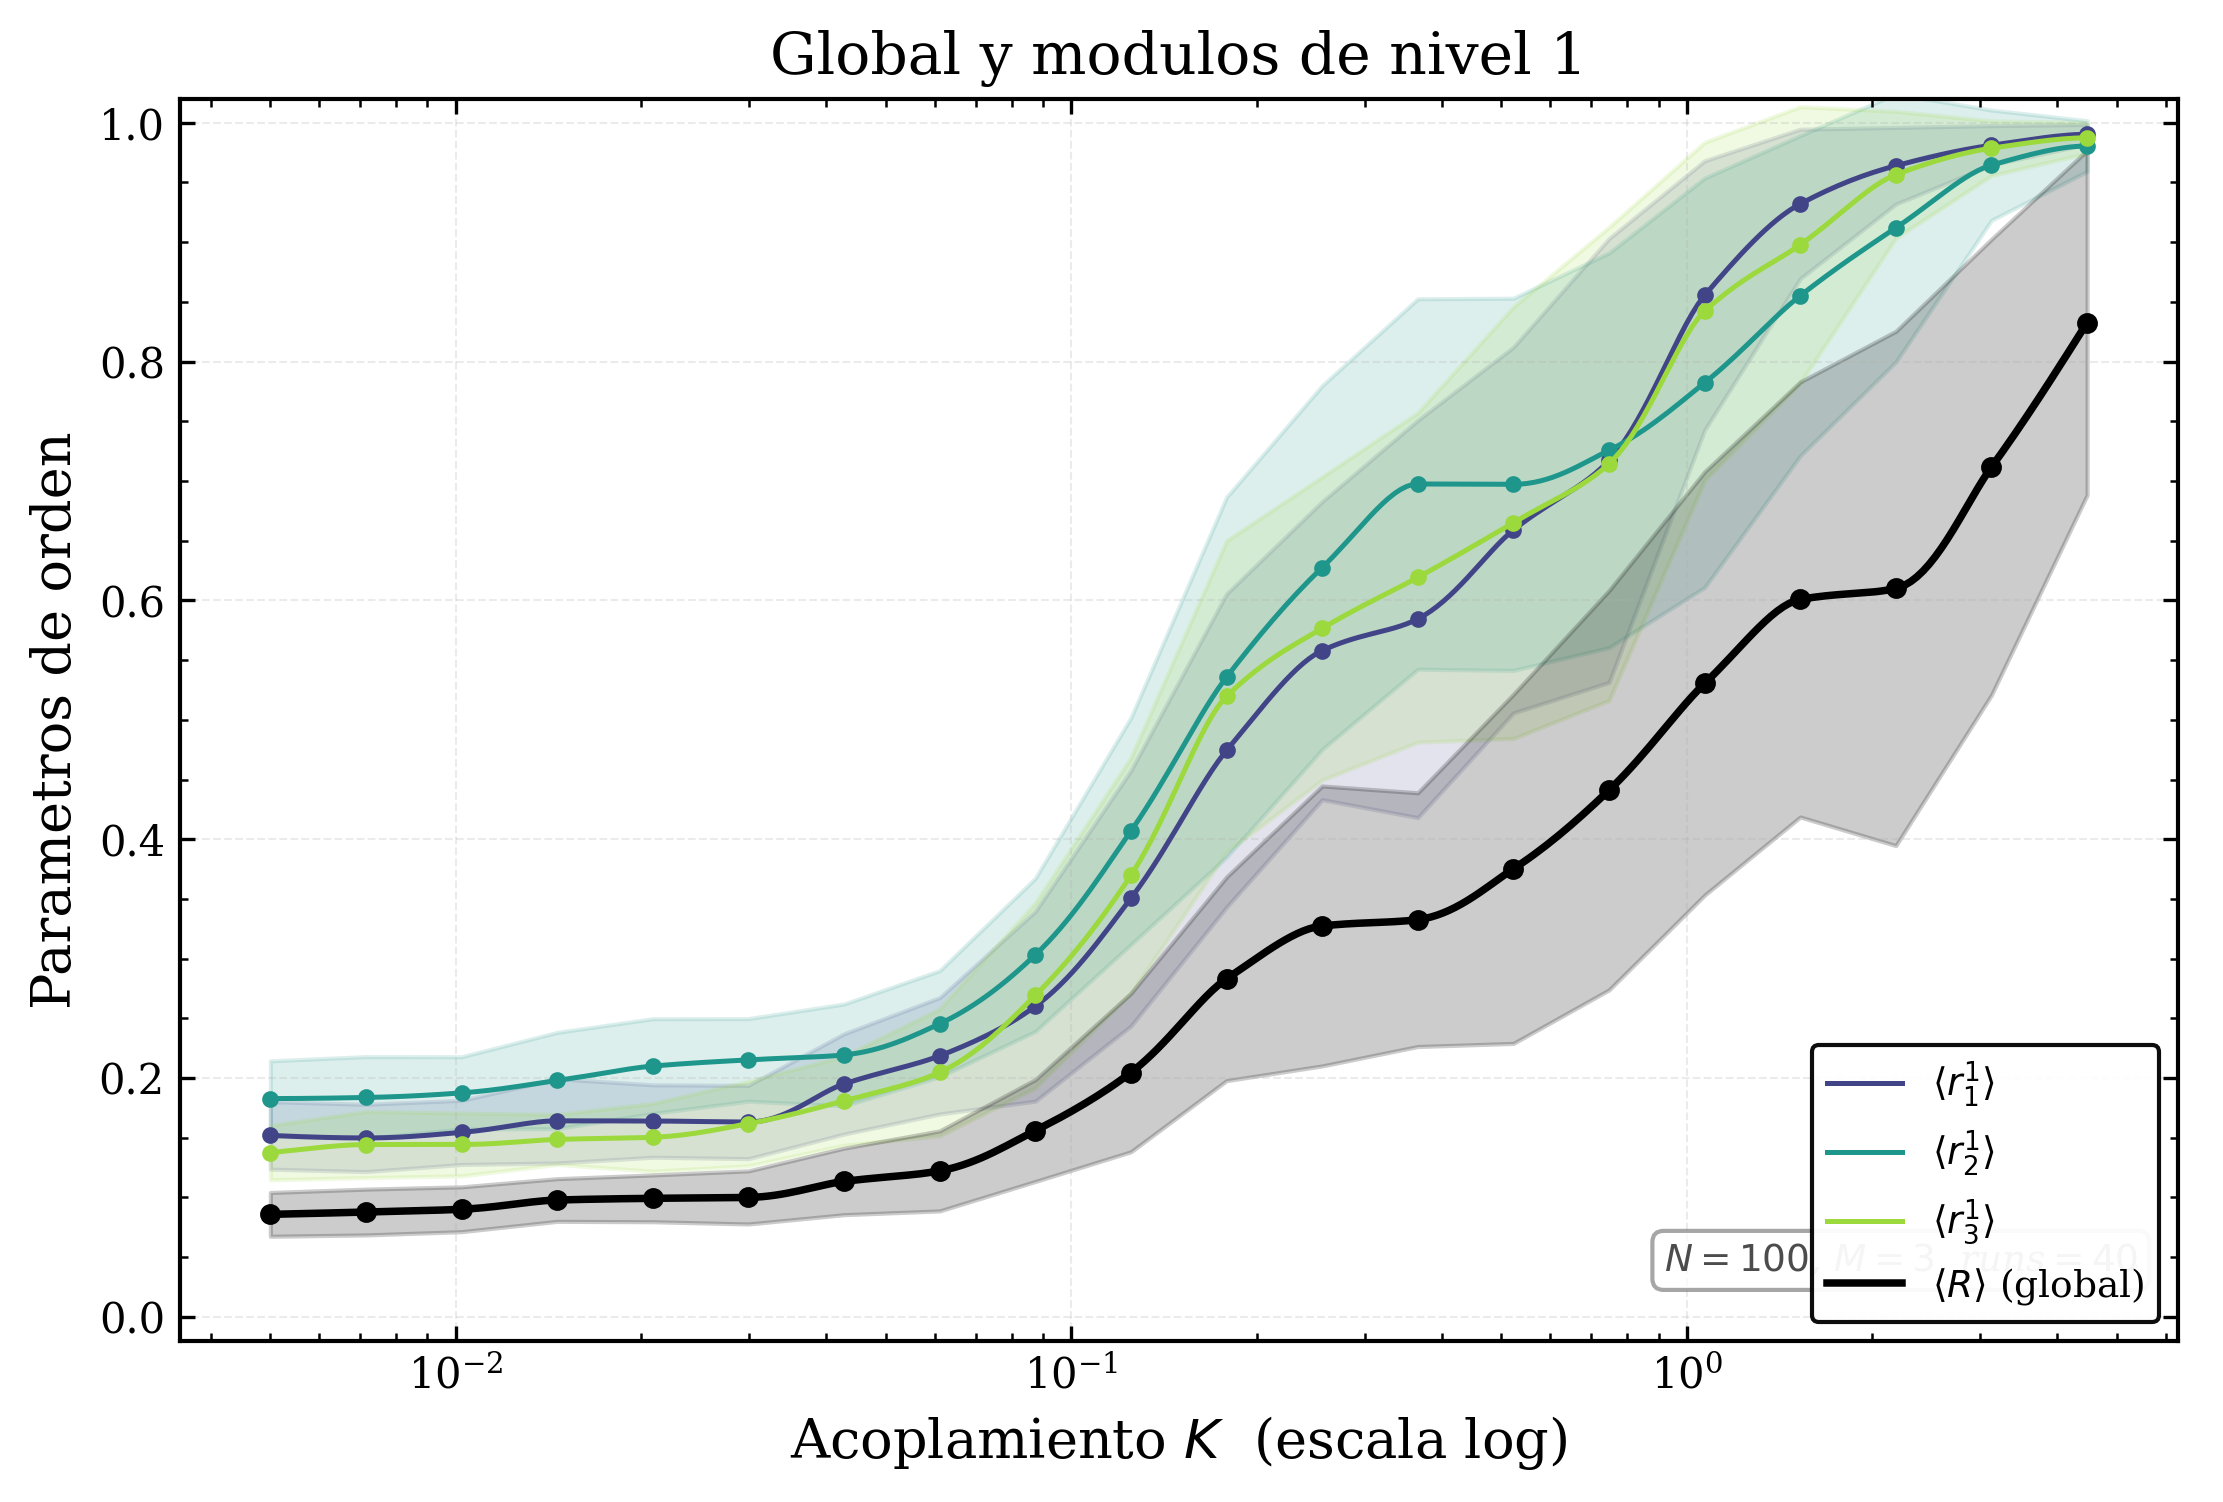
\includegraphics[width=0.45\textwidth]{Rglobal_nivel1.png}\hfill
  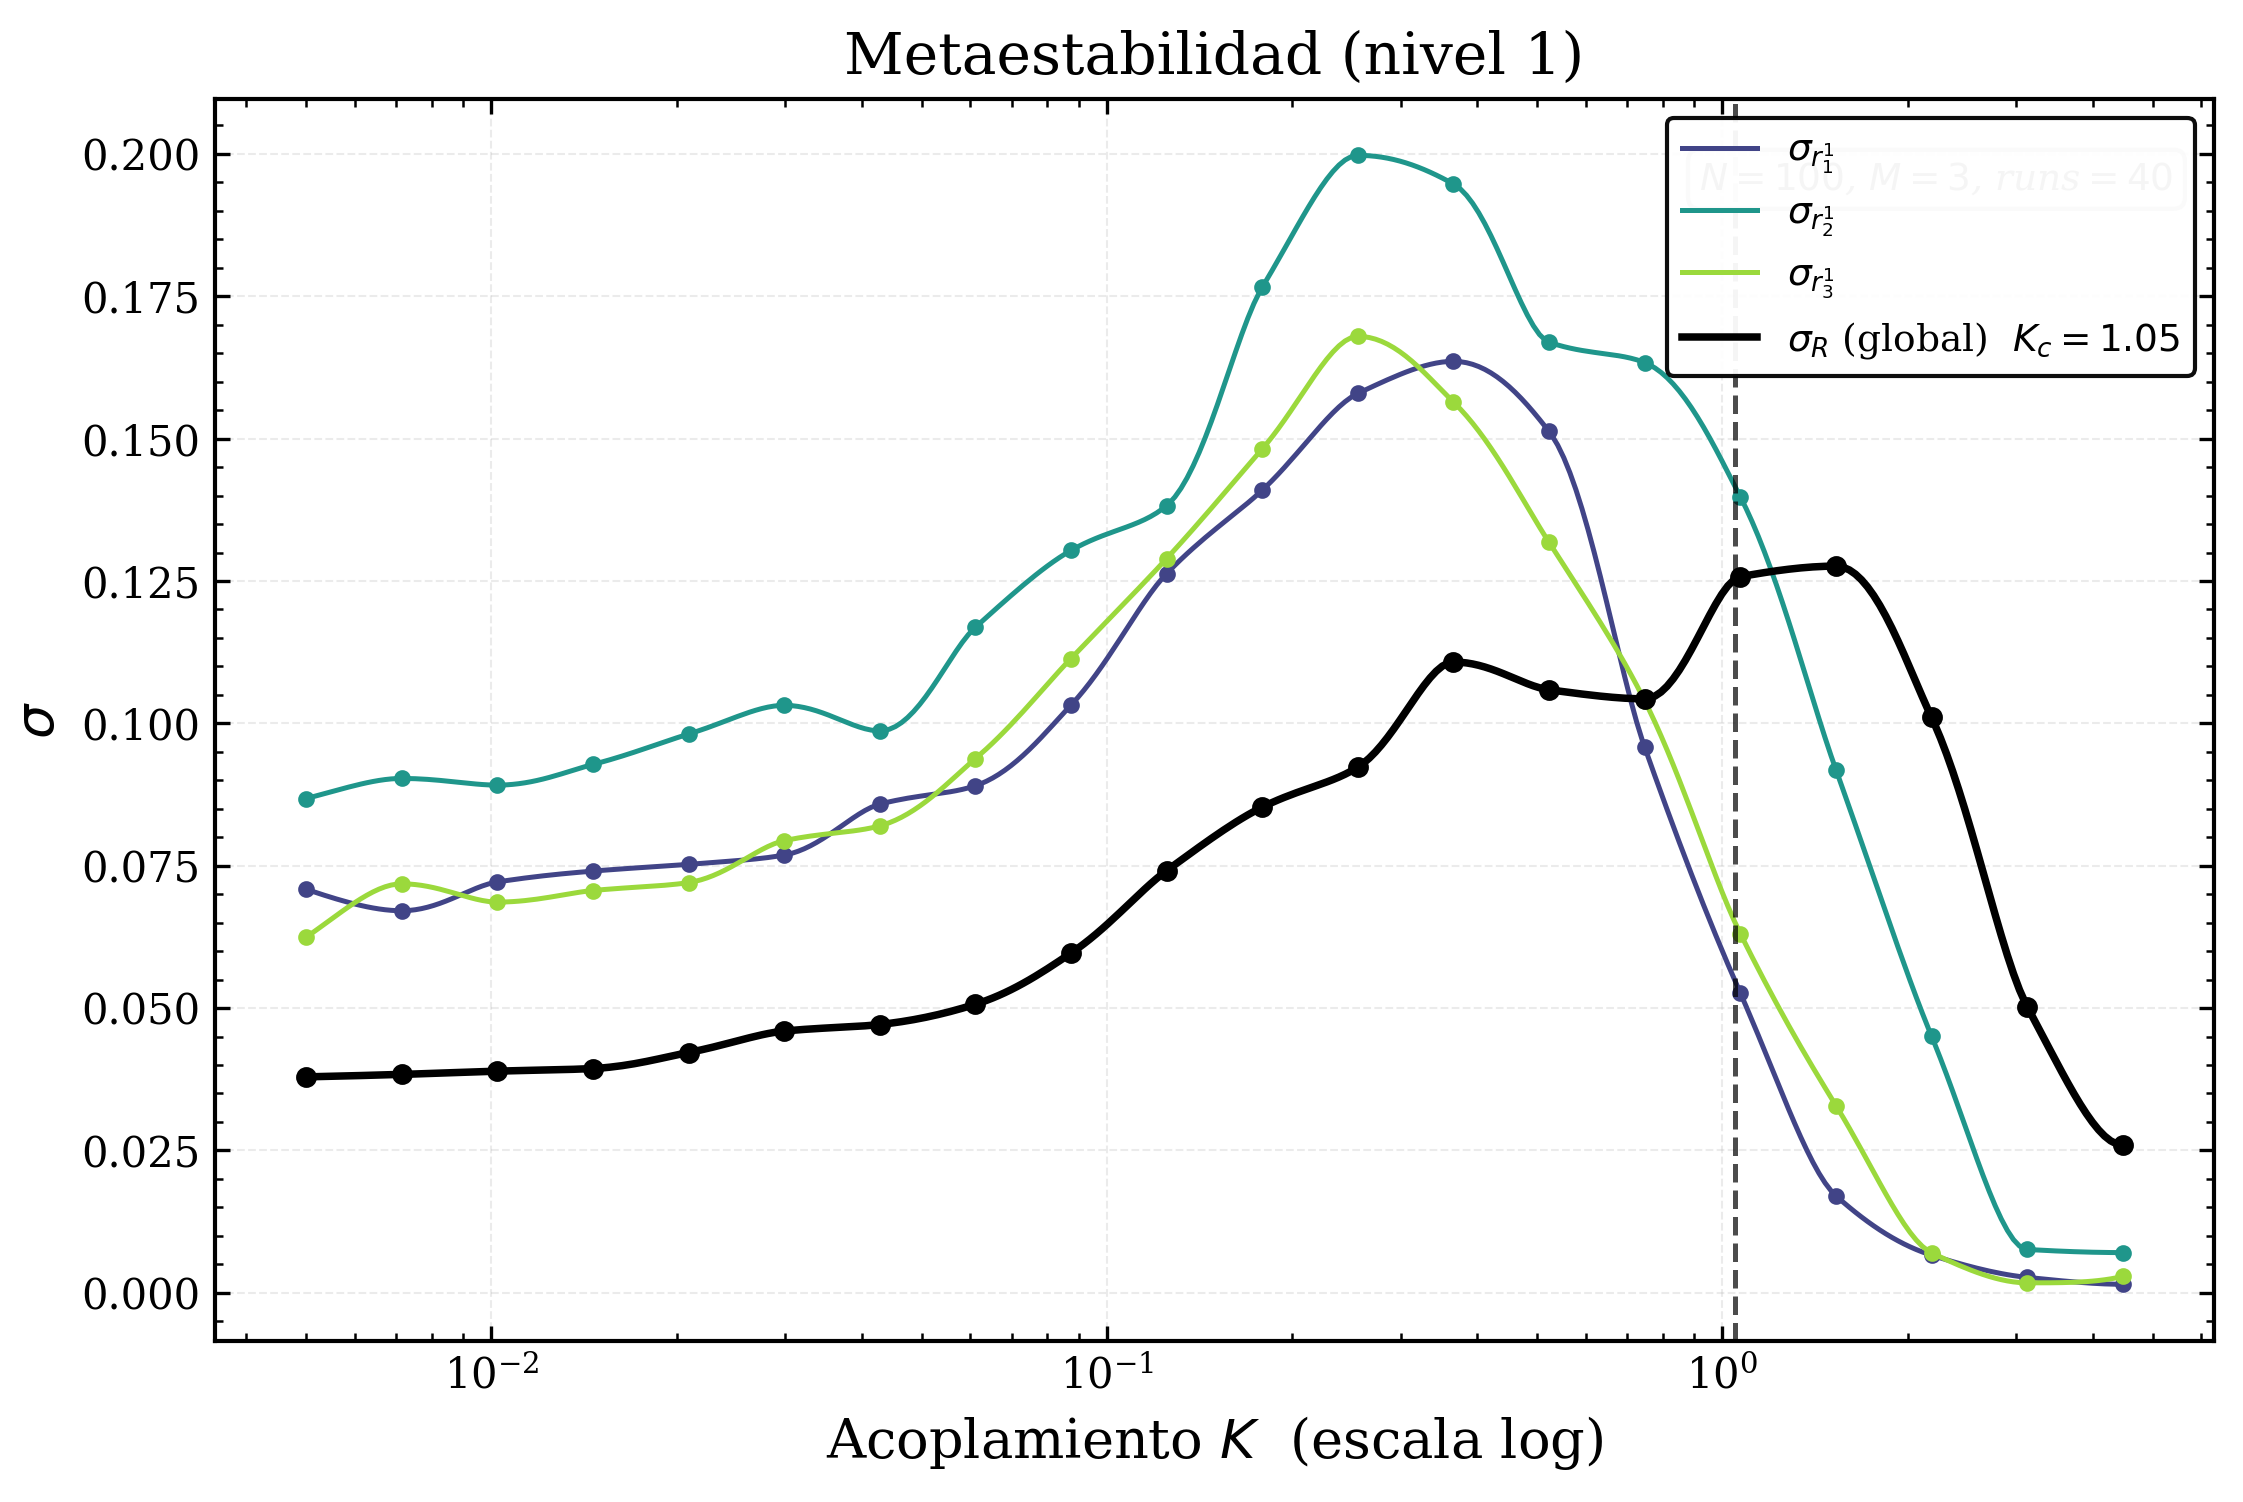
\includegraphics[width=0.45\textwidth]{sigmaglobal_nivel1.png}
  \caption{Visión global de la red jerárquica. Izquierda: en negro, promedio del parámetro de orden global $\langle R\rangle$ frente a $K$; en azul, turquesa y verde, parámetros de orden de los módulos de nivel 1, $\langle r_1^1\rangle$, $\langle r_2^1\rangle$ y $\langle r_3^1\rangle$. Derecha: en negro, desviación estándar del parámetro de orden global $\sigma_R$ frente a $K$; en azul, turquesa y verde, $\sigma_{r_1^1}$, $\sigma_{r_2^1}$ y $\sigma_{r_3^1}$. Se muestra también el valor crítico $K_c$ obtenido como el máximo de $\sigma_R$ global (mediante un ajuste cuadrático alrededor del pico).}
  \label{fig:tarea3_global}
\end{figure*}

\subsection{Tarea 4: hacia redes tipo cerebro}
\label{sec:tarea4}

La última etapa consiste en sustituir las redes sintéticas por la matriz de conectividad estructural obtenida del promedio de 88 sujetos sanos (atlas AAL, 90 regiones). Como control se genera una red aleatoria que preserva el grado de cada nodo mediante \textit{double-edge swaps}, de modo que cualquier diferencia observable se atribuye al patrón de conectividad y no a la distribución de grados.

Ambas redes exhiben una transición desde un estado incoherente ($R\approx 0.1$) hasta sincronización total ($R\approx 1$), con curvas globalmente similares (\cref{fig:t4_bin}). Sin embargo, la transición del conectoma aparece ligeramente desplazada hacia valores mayores de $K$ respecto a la red aleatoria, lo que indica que la topología real del cerebro ofrece mayor resistencia a la sincronización global. El pico de $\sigma_R$ del conectoma ($K_c = 0.0615$) es más alto y está desplazado a la derecha respecto al de la red aleatoria ($K_c = 0.0506$). Además, la curva del conectoma presenta una región de fluctuaciones elevadas ($\sigma_R \approx 0.05$) sostenida en un rango amplio de $K$ antes del pico principal, algo ausente en la red aleatoria, cuya $\sigma_R$ crece de forma más suave hasta su máximo. Esta meseta previa al pico es la firma de la metaestabilidad: la red real mantiene un régimen prolongado de sincronización parcial antes de alcanzar la coherencia global.

El desglose hemisférico (\cref{fig:t4_bin_hemi}) reproduce el patrón observado en las redes modulares y jerárquicas: los parámetros de orden hemisféricos crecen antes que el global, indicando que cada hemisferio alcanza coherencia interna a valores de $K$ para los que el sistema como conjunto permanece parcialmente incoherente. Las bandas de error, notablemente anchas en la región de transición, reflejan la alta variabilidad entre realizaciones propia del régimen metaestable. Las desviaciones estándar hemisféricas ($\sigma_{r_{\rm izq}}$, $\sigma_{r_{\rm der}}$) alcanzan valores de hasta $\sigma \approx 0.10$, superiores al máximo de $\sigma_R \approx 0.08$, y sus picos se sitúan a valores de $K$ ligeramente inferiores al del parámetro global. Este desfase entre las escalas de fluctuación local y global es cualitativamente análogo al observado en la red modular de dos módulos (\cref{fig:tarea2}) y en la red jerárquica (\cref{fig:tarea3_global}), pero aquí emerge de la estructura anatómica real del conectoma sin haber sido impuesto por construcción.

\begin{figure*}[t]
  \centering
  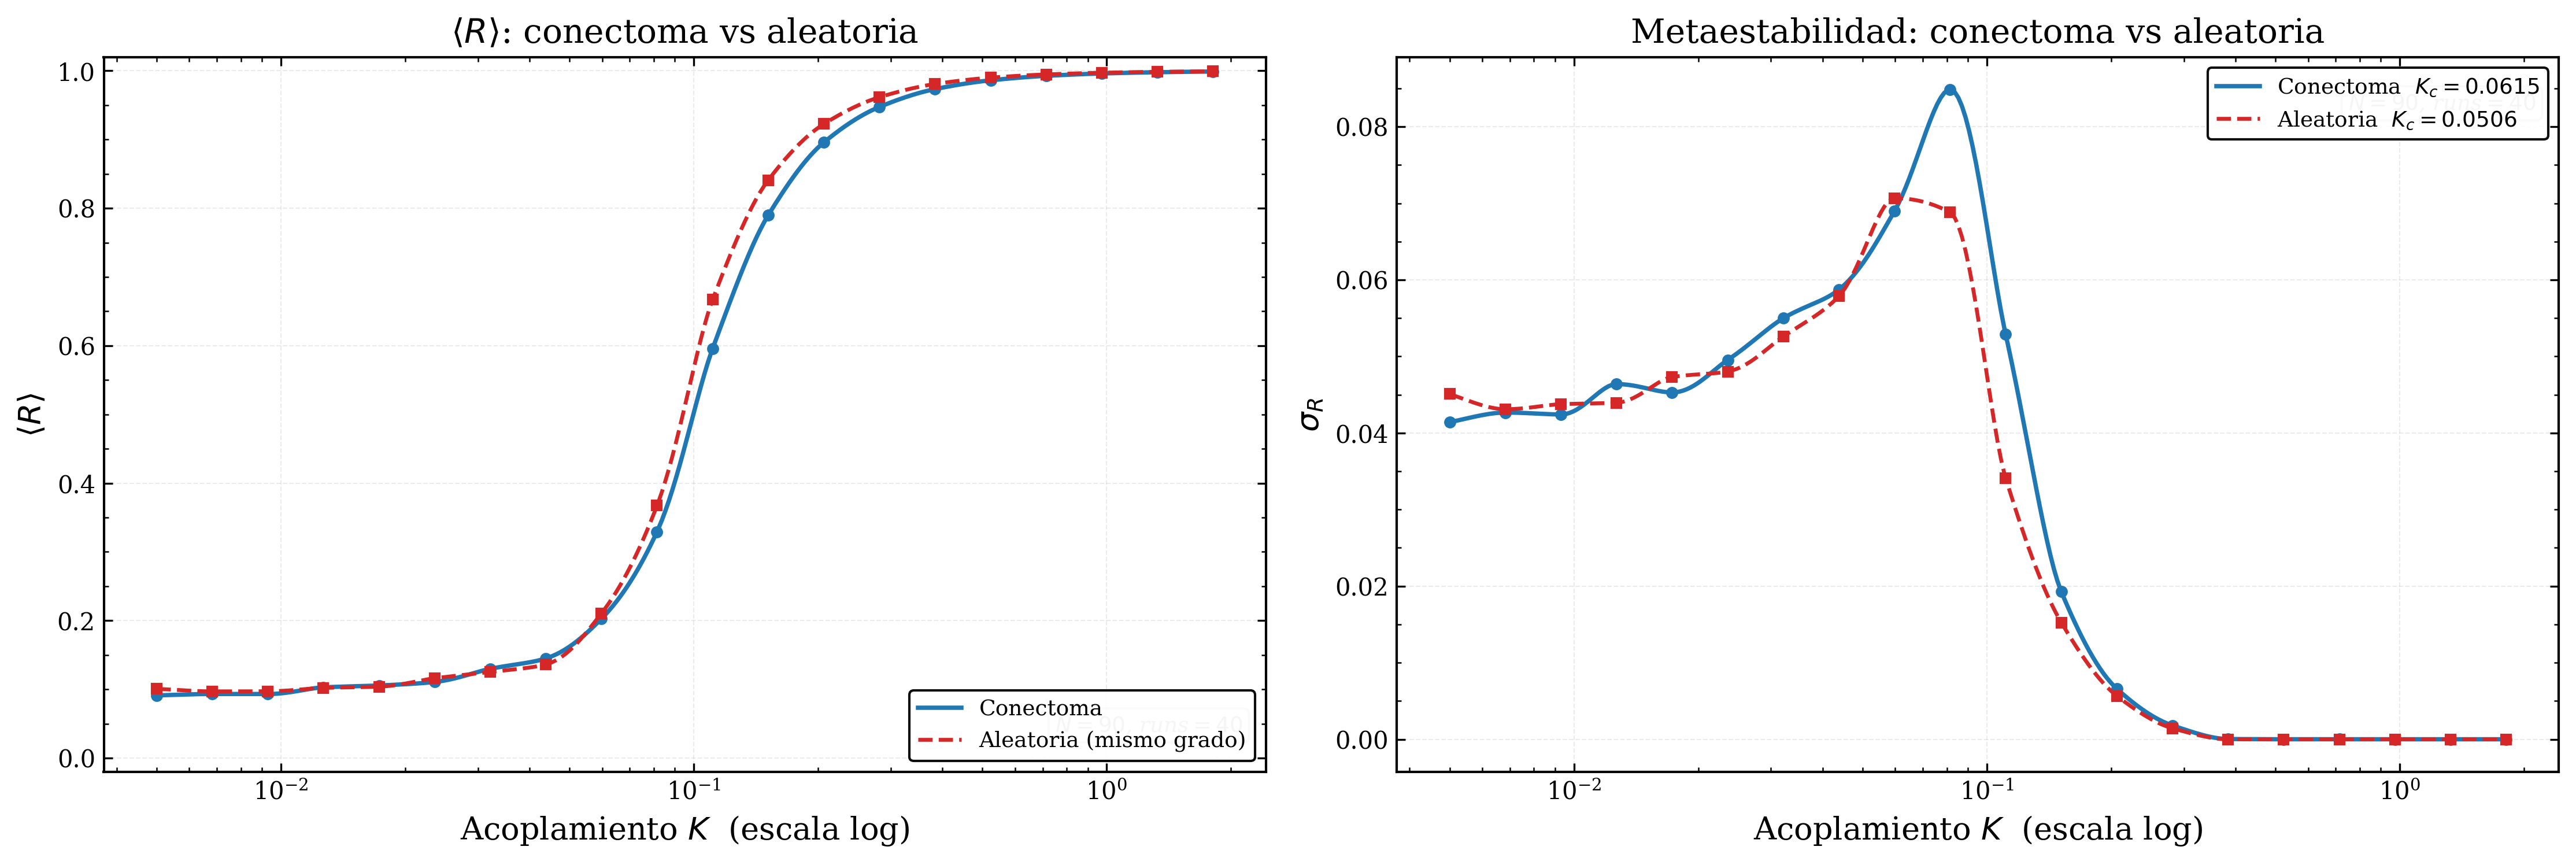
\includegraphics[width=0.9\textwidth]{Conect_vs_Aleat_bin.png}
  \caption{Conectoma binarizado: comparación con la red aleatoria que preserva el grado. Izquierda: promedio del parámetro de orden global $\langle R\rangle$ frente a $K$ para el conectoma real (azul) y la red aleatoria (rojo). Derecha: desviación estándar $\sigma_R$ frente a $K$, con los valores de $K_c$ correspondientes.}
  \label{fig:t4_bin}
\end{figure*}

\begin{figure*}[t]
  \centering
  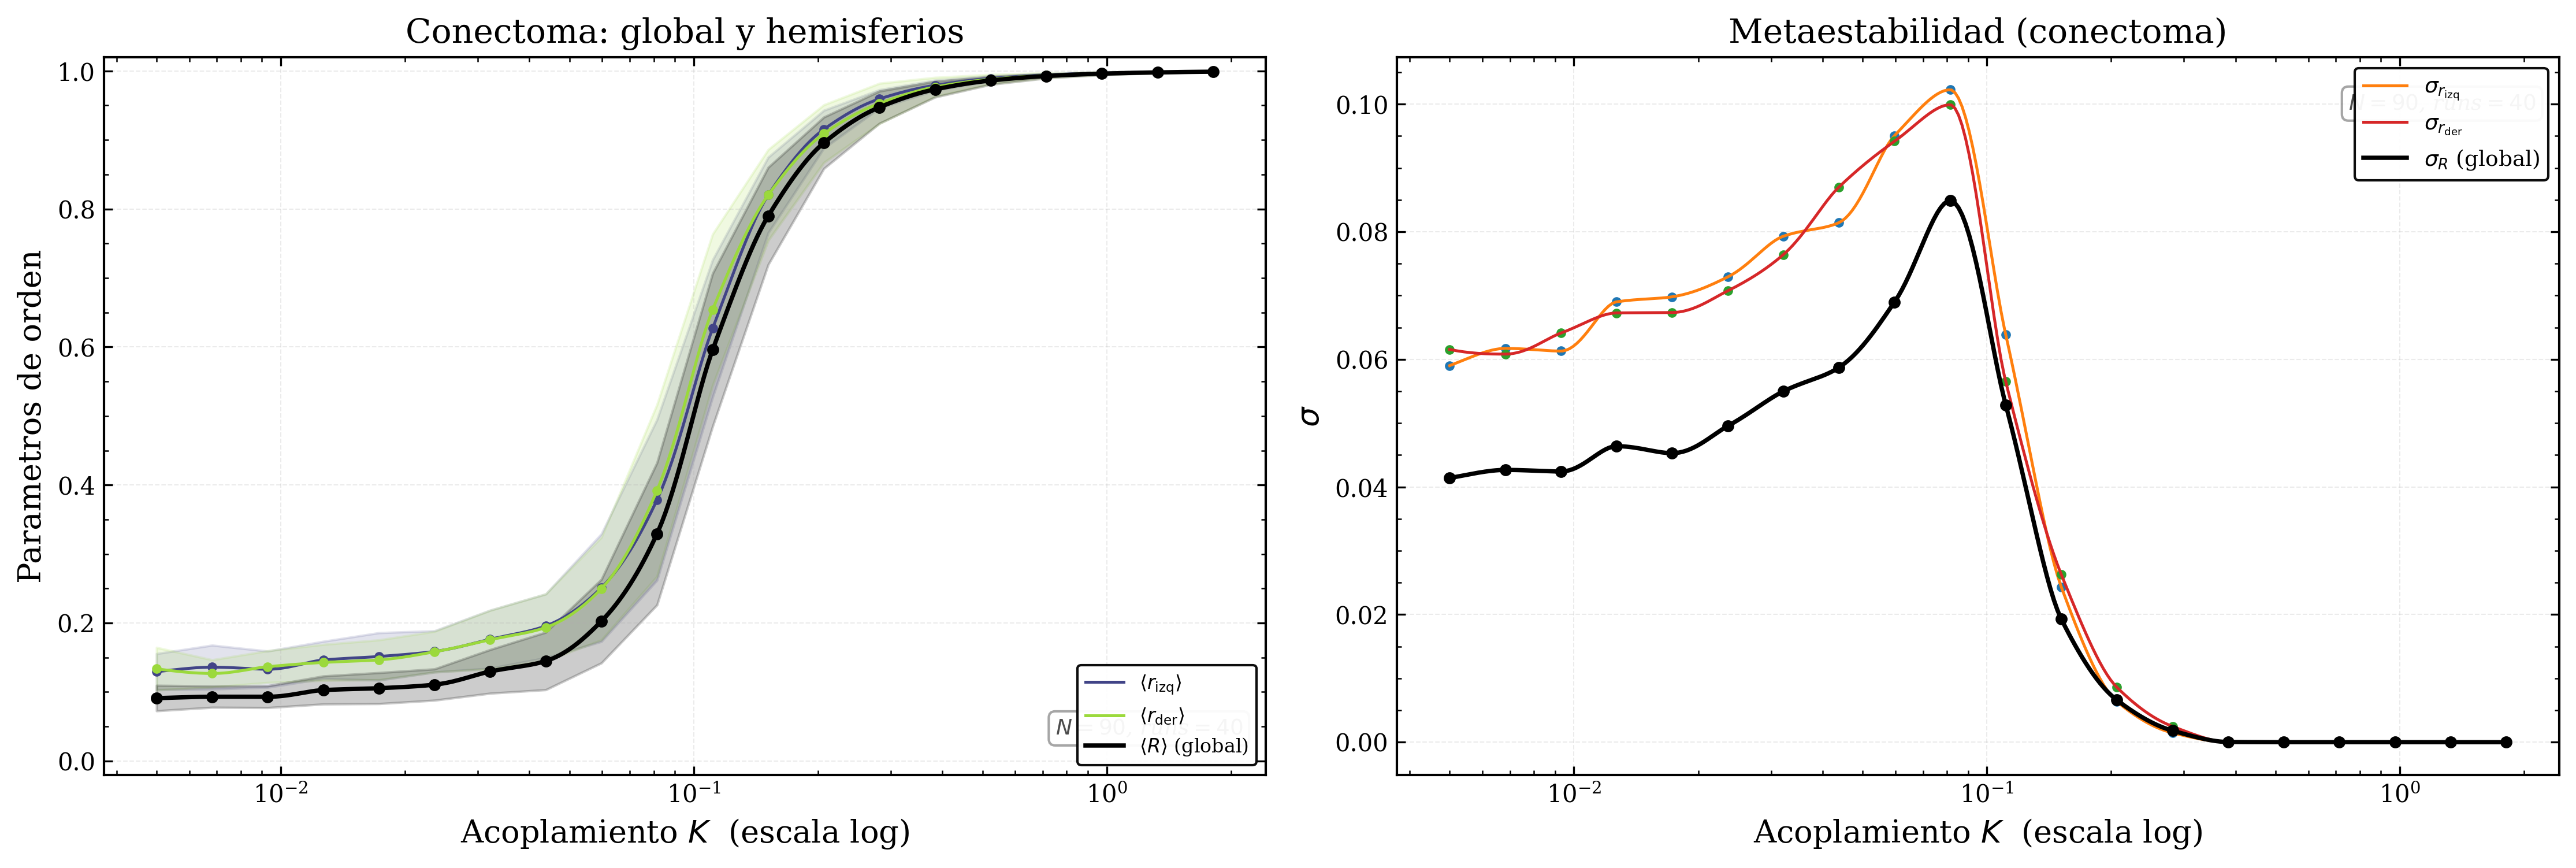
\includegraphics[width=0.9\textwidth]{Conect_r_vs_K_bin.png}
  \caption{Conectoma binarizado: desglose hemisférico. Izquierda: promedio de los parámetros de orden hemisféricos $\langle r_{\rm izq}\rangle$ y $\langle r_{\rm der}\rangle$ junto al global $\langle R\rangle$, en función de $K$; las bandas sombreadas indican la desviación estándar entre realizaciones. Derecha: desviaciones estándar $\sigma_{r_{\rm izq}}$, $\sigma_{r_{\rm der}}$ y $\sigma_R$ frente a $K$.}
  \label{fig:t4_bin_hemi}
\end{figure*}

Al introducir pesos discretizados en 5 niveles en lugar de la matriz binaria, las diferencias entre el conectoma y la red aleatoria se amplifican de forma notable (\cref{fig:t4_disc}). La red aleatoria alcanza sincronización total ($R\approx 1$) en torno a $K\approx 10$, mientras que el conectoma apenas llega a $\langle R\rangle \approx 0.8$ en el extremo del barrido, sin completar la transición. La separación entre ambas curvas, apenas perceptible en la versión binaria, abarca aquí más de una década en $K$. El acoplamiento crítico del conectoma ($K_c = 2.14$) es más del doble que el de la red aleatoria ($K_c = 0.985$). Además, la curva $\sigma_R$ del conectoma sostiene un nivel elevado de fluctuaciones ($\sigma_R \approx 0.05$--$0.07$) a lo largo de un rango amplio de $K$ antes de alcanzar su máximo, configurando una región metaestable mucho más extendida que la que presenta la red aleatoria, cuyo pico es más estrecho y localizado.

El desglose hemisférico (\cref{fig:t4_disc_hemi}) confirma la tendencia. Los parámetros de orden hemisféricos $\langle r_{\rm izq}\rangle$ y $\langle r_{\rm der}\rangle$ crecen por delante del global, pero la separación entre las curvas locales y la global es ahora mayor que en el caso binario, y las bandas de error son considerablemente más anchas, reflejando una variabilidad entre realizaciones propia de un régimen metaestable más intenso. Las desviaciones estándar hemisféricas alcanzan valores de hasta $\sigma \approx 0.115$, claramente por encima del máximo global ($\sigma_R \approx 0.08$), y presentan sus picos a valores de $K$ inferiores al del parámetro global. La heterogeneidad introducida por los pesos discretos ---que distingue conexiones fuertes de débiles--- amplifica notablemente la metaestabilidad del conectoma frente a la red aleatoria, un efecto que apenas se insinuaba en la versión binaria. La tendencia es clara: cuanto más fielmente se recoge la distribución de pesos sinápticos, más favorece la red la coexistencia de módulos localmente coherentes pero globalmente desacoplados. Esto es consistente con la hipótesis de que la arquitectura del conectoma humano está organizada de forma que favorece activamente la metaestabilidad como régimen funcional. La red aleatoria, al destruir esta organización manteniendo solo la estadística de grados, pierde precisamente esa capacidad, lo que confirma que es la topología específica del conectoma, y no su distribución de grados, la responsable de la potenciación observada.

\begin{figure*}[t]
  \centering
  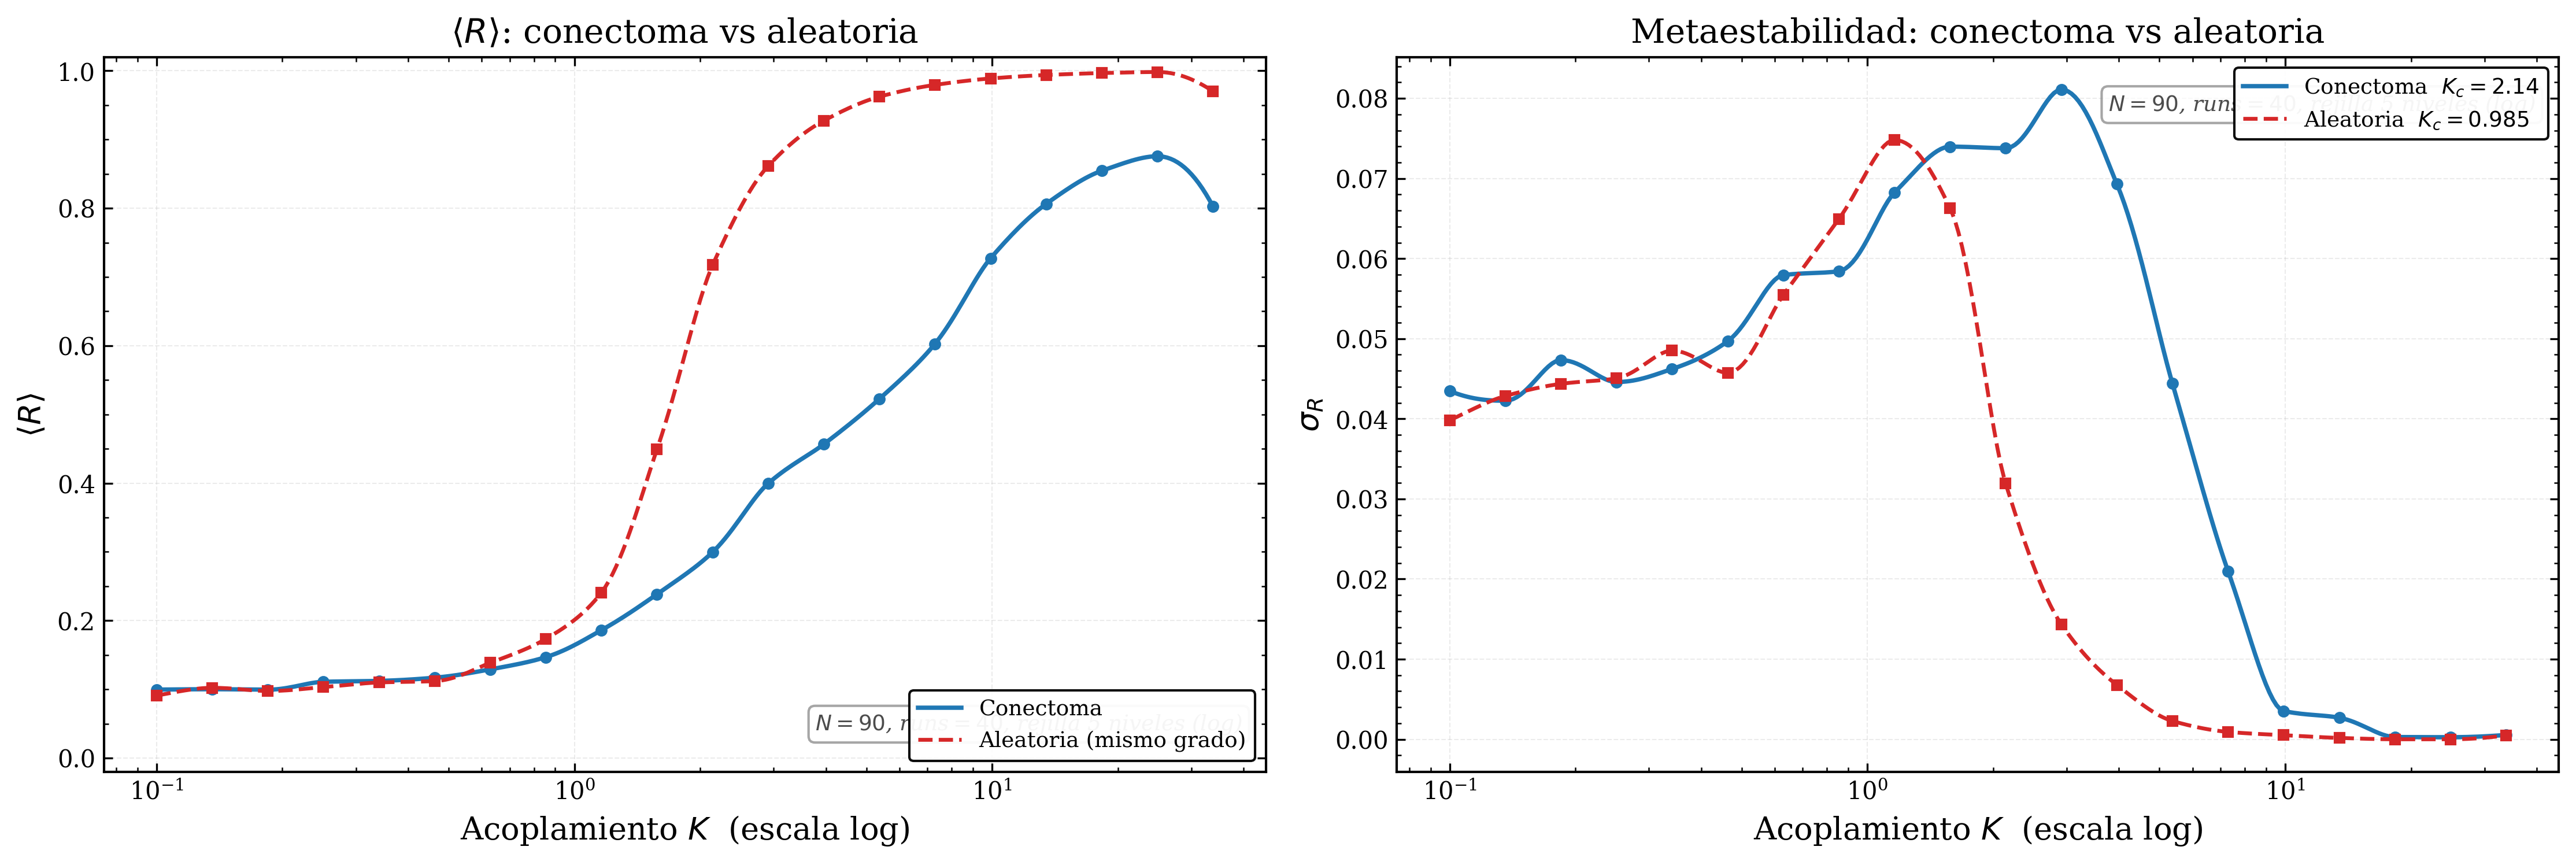
\includegraphics[width=0.9\textwidth]{Conect_vs_Aleat_dicrete.png}
  \caption{Conectoma discretizado en 5 niveles: comparación con la red aleatoria. Izquierda: $\langle R\rangle$ frente a $K$ para el conectoma real (azul) y la red aleatoria (rojo). Derecha: $\sigma_R$ frente a $K$, con los valores de $K_c$ correspondientes.}
  \label{fig:t4_disc}
\end{figure*}

\begin{figure*}[t]
  \centering
  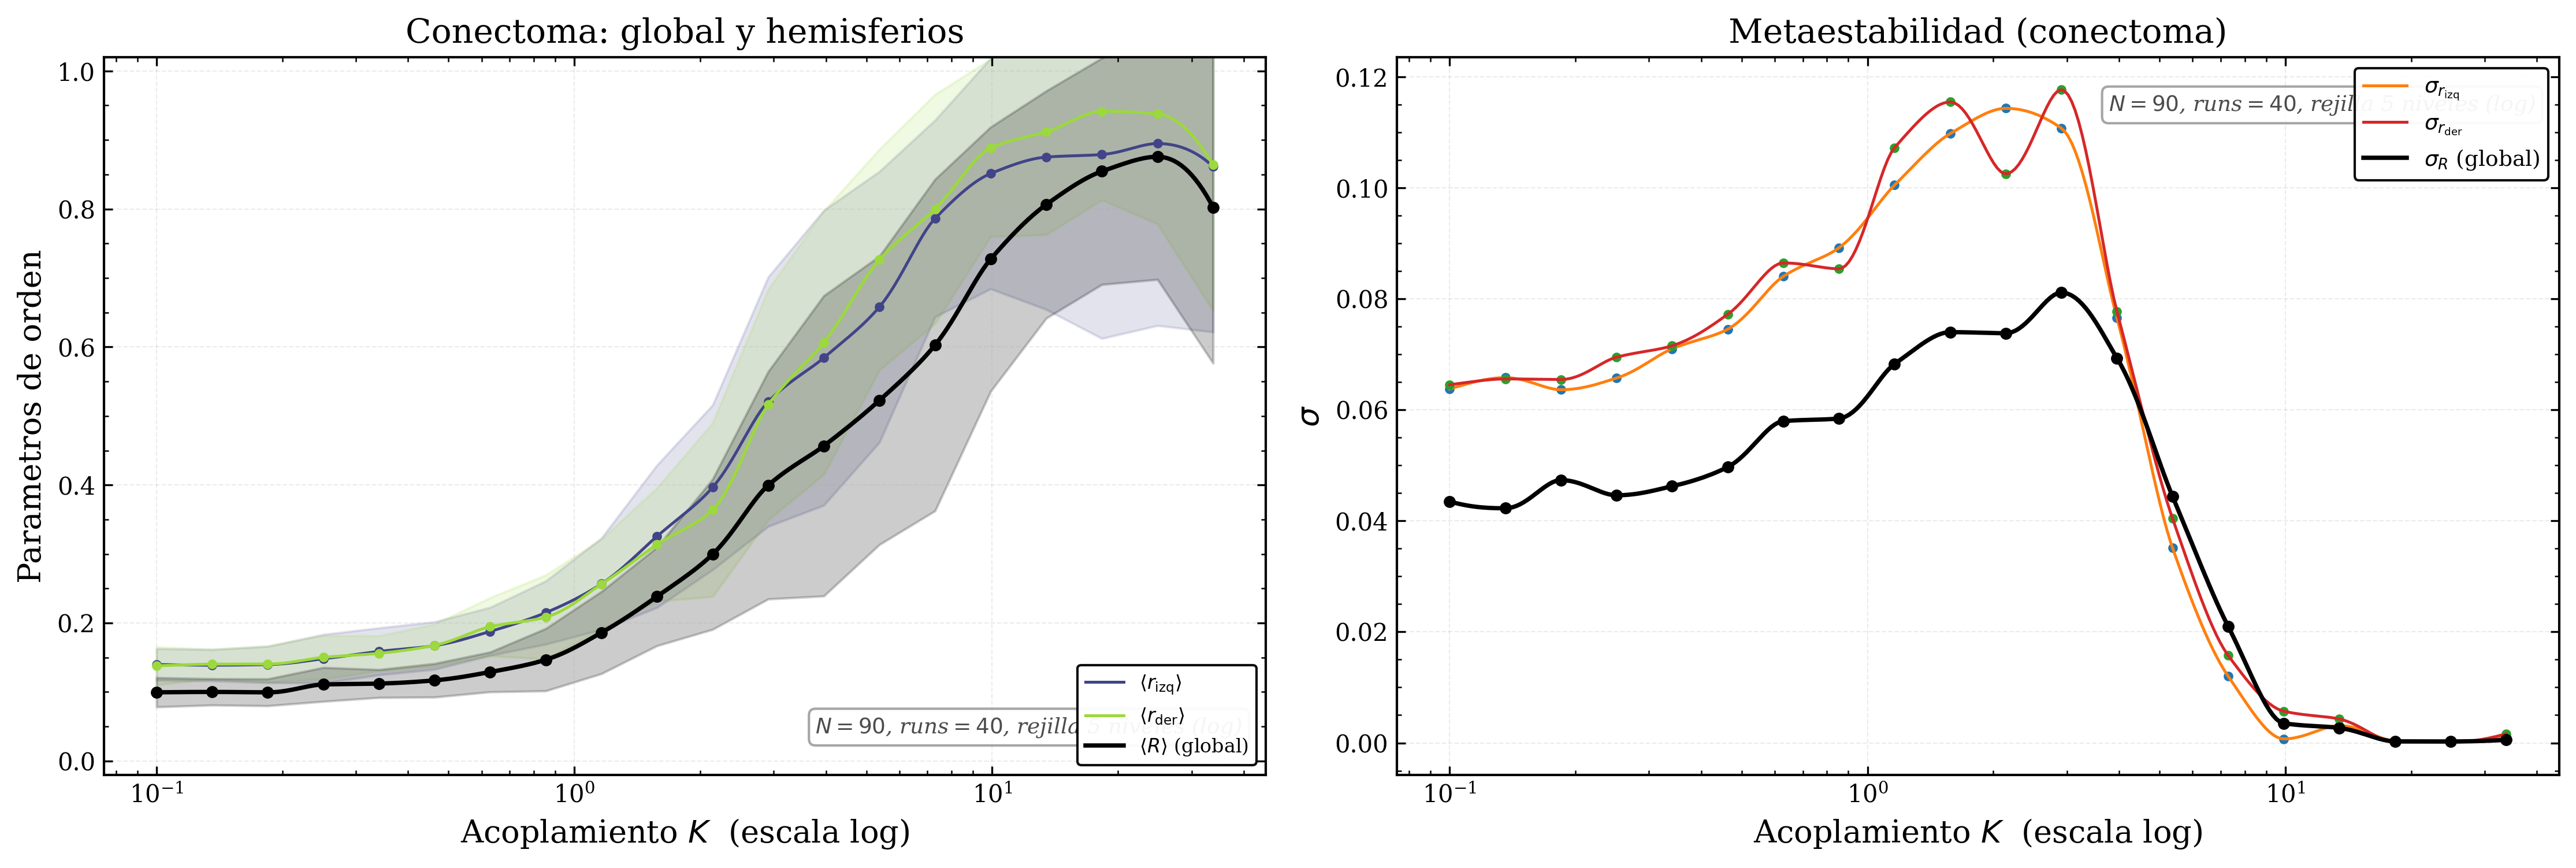
\includegraphics[width=0.9\textwidth]{Conect_r_vs_K_discrete.png}
  \caption{Conectoma discretizado en 5 niveles: desglose hemisférico. Izquierda: promedio de los parámetros de orden hemisféricos $\langle r_{\rm izq}\rangle$ y $\langle r_{\rm der}\rangle$ junto al global $\langle R\rangle$, en función de $K$; las bandas sombreadas indican la desviación estándar entre realizaciones. Derecha: desviaciones estándar $\sigma_{r_{\rm izq}}$, $\sigma_{r_{\rm der}}$ y $\sigma_R$ frente a $K$.}
  \label{fig:t4_disc_hemi}
\end{figure*}

% =============================================================================
% 4. Discusion y conclusiones
% =============================================================================
\section{Discusión y conclusiones}
\label{sec:conclusiones}

En este trabajo hemos construido progresivamente un modelo de Kuramoto desde la configuración más sencilla ---campo medio--- hasta la conectividad anatómica real del cerebro humano, analizando en cada etapa cómo la topología de la red modifica los regímenes de sincronización accesibles.

La transición clásica de campo medio (Tarea 1) reproduce fielmente la predicción teórica $K_c^{\rm teo} = 2/[\pi g(0)]$, con errores relativos inferiores al $5\%$, y el análisis de escalado de tamaño finito confirma la ley $K_c(N) = K_c^\infty + a\,N^{-2/5}$ propuesta por Hong \textit{et al.}~\cite{hong2007finite}. Este régimen sirve como referencia: la transición es abrupta, el pico de $\sigma_R$ es estrecho y no hay metaestabilidad.

La introducción de estructura modular (Tarea 2) cambia cualitativamente el panorama. La débil conexión inter-modular genera un régimen metaestable extendido en $K$, donde cada módulo alcanza coherencia interna pero el sistema global permanece parcialmente incoherente. El pico estrecho de $\sigma_R$ se ensancha en un plateau, y las fluctuaciones macroscópicas sostenidas del parámetro de orden global reflejan la frustración entre las escalas local y global. La red jerárquica (Tarea 3) añade un nivel de complejidad: la sincronización emerge de forma escalonada, consolidándose primero en los submódulos, después en los módulos y finalmente a escala global, dando lugar a múltiples mesetas de metaestabilidad.

Al pasar al conectoma real (Tarea 4), todos estos fenómenos reaparecen sin haber sido impuestos por construcción. La comparación con la red aleatoria que preserva la distribución de grados demuestra que es la topología específica del conectoma ---y no simplemente su heterogeneidad de grados--- la responsable de potenciar la metaestabilidad. Este efecto se intensifica al pasar de la representación binaria a la discretizada en 5 niveles: el $K_c$ del conectoma se desplaza significativamente respecto al de la red aleatoria, la región metaestable se ensancha y las fluctuaciones hemisféricas superan ampliamente a las globales. La organización modular y jerárquica del cerebro, combinada con la distribución heterogénea de pesos sinápticos, favorece de forma natural un régimen donde coexisten módulos localmente coherentes pero globalmente desacoplados.

Estos resultados son consistentes con la visión de que la metaestabilidad no es un artefacto del modelo, sino un régimen funcional del cerebro~\cite{cabral2011role,villegas2014frustrated}: un estado que permite flexibilidad dinámica, facilitando la integración y segregación simultánea de información entre regiones cerebrales. Las anomalías en este equilibrio ---exceso o déficit de sincronización--- conectan directamente con las patologías descritas por Uhlhaas y Singer~\cite{uhlhaas2006neural}, cerrando el arco que motivaba este trabajo.

Entre las limitaciones, cabe señalar que el modelo empleado es puramente de fase (sin amplitud), no incluye retardos de conducción axonal ni ruido, y la asignación de frecuencias naturales por región es una aproximación simplificada de la actividad oscilatoria real. Extensiones naturales incluirían el modelo de Kuramoto-Sakaguchi con frustración explícita, retardos dependientes de la distancia anatómica y la comparación con datos de conectividad funcional obtenidos por fMRI.


% =============================================================================
% Bibliografia
% =============================================================================
\bibliography{Referencias}

\end{document}